% !Mode:: "TeX:UTF-8"

\documentclass[bachelor]{uestcthesis}
\usepackage{IEEEtrantools}
\usepackage{algorithm}
\usepackage{algorithmic}
\usepackage{multirow}
\usepackage{indentfirst}
\title{基于同步原理的多边聚类算法研究}
\author{高崇铭}
\date{2013}{4}{15}
\begin{document}
\newcommand{\red}[1]{{\textcolor{red}{{} #1}}}
\newcommand{\ud}{\,\mathrm{d}}
\newcommand{\bt}{\vrule width 0.85pt}
\newcommand{\CoSync}{CoSync}
\newcommand{\Sync}{Sync}
\newcommand{\cosync}{CoSync}
\newcommand{\sync}{Sync}
\makeatletter
\def\hlinew#1{%
  \noalign{\ifnum0=`}\fi\hrule \@height #1 \futurelet
   \reserved@a\@xhline}

% !Mode:: "TeX:UTF-8"

\chapter{绪论}
\section{引言-从数据挖掘谈起}
% 计算电磁学方法\citeup{wang1999sanwei,
% liuxf2006,
% zhu1973wulixue,
% chen2001hao,
% gu2012lao,
% feng997he}
% 从时、频域角度划分可以分为频域方法与时域方法两大类。
% 频域方法的研究开展较早,目前应用广泛的包括:矩量法(MOM)\citeup{xiao2012yi,zhong1994zhong}及其快速算
% 法多层快速多极子(MLFMA)\citeup{clerc2010discrete}方法、有限元(FEM)\citeup{wang1999sanwei,zhu1973wulixue}方法、自适应积分(AIM)
% \citeup{gu2012lao}方法等,这些方法是目前计算电磁学商用软件
% \footnote{脚注序号“①,……,⑩”的字体是“正文”,不是“上标”,序号与脚注内容文字之间空1个半角字符,脚注的段落格式为:单倍行距,段前空0磅,段后空0磅,悬挂缩进1.5字符;中文用宋体,字号为小五号,英文和数字用Times New Roman字体,字号为9磅;中英文混排时,所有标点符号(例如逗号“,”、括号“()”等)一律使用中文输入状态下的标点符号,但小数点采用英文状态下的样式“.”。}
% (例如:FEKO、Ansys 等)的
% 核心算法。由文献\cite{feng997he,clerc2010discrete,xiao2012yi}可知……
现如今,我们处于一个充满数据的时代。在每一天我们使用计算机、手机时候,都有大量数据产生,接着被以各种形式记录、保留下来。许多数据都给我们的生活提供着极大的便利,比如根据用户的音乐的历史记录,音乐软件能推荐更多的适合该客户口味的音乐;再比如当我用键盘输入这段文字的时候,中文输入软件根据词库里的数据,将键入的字母序列转换为一段段可能性最大的中文词汇或句子。在经济学、医学、生物学、社会科学等学科中,海量的数据无时无刻不在产生,然而如何合理地利用这些数据,使其提供我们需要的信息,成为了现在各个领域面临的问题。

在这样多领域的需求下,数据挖掘(Data Mining,缩写:DM)这门交叉学科应运而生。通常来说,数据挖掘是数据库知识发现(Knowledge-Discovery in Databases,缩写:KDD)中的一个步骤,其目的是在大量的数据中自动搜索隐藏于其中的特殊信息,从而为之后的分析决策提供理论依据。下面将简要介绍下数据挖掘的主要步骤:
\vspace{4mm}
\pic[h]{RWG 基函数几何参数示意图}{}{overview}
\begin{itemize}
    \item \textbf{~~数据采集} 首先需要采集数据,包括确定数据种类、范围等。
    \item \textbf{~~数据预处理} 该过程包括对原始数据的处理,包括数据整合、去除噪声等。
    \item \textbf{~~数据表示} 对数据进行完预处理后,需要决定数据合适表示,例如特征选筛等。
    \item \textbf{~~数据挖掘} 这个过程中,人们采用各种方法,例如聚类、分类、关联规则分析等方法来发掘数据中的有用的信息。
    \item \textbf{~~结果解析与评估} 最后,需要对得到的结果进行解释与评估,有可能需要重新进行挖掘。
\end{itemize}

\vspace{2mm}
这其中,\textbf{数据挖掘}是从数据中学习知识的最关键的步骤,因此很多时候,数据挖掘泛指从数据中学习知识的过程。数据挖掘的大量算法可以按照目的分为以下四类:

\begin{itemize}
    \item \textbf{~~分类} 分类算法的目的是为特定变量确定类别或者标签,比如根据近年来我国的经济发展情况来确定房价是涨还是跌。一般来说,分类首先用历史数据作为训练集,学习出目标函数,然后用学到的目标函数来预测新来的未知数据点的类别。常见的分类算法有\emph{kNN}\cite{peterson2009k},\emph{决策树}\cite{quinlan1986induction},\emph{支持向量机}\cite{cortes1995support}等。
    \item \textbf{~~聚类} 聚类算法的目的是将数据分为许多类,使得相似的数据分在同一类中,不相似的数据分布在不同的类中,比如菜农可以根据一批辣椒的形状、辛辣程度将其聚拢成不同类别销售。常见的聚类方法有\emph{k-means}\cite{hartigan1979algorithm}, \emph{spectral clustering}\cite{ng2002spectral} 等方法。
    \item \textbf{~~关联规则分析} 关联规则分析的目的是从数据中发现经常出现的模式,一个经典的例子是人们从超市的大量销售记录中发现买尿布的人也常常买啤酒。经典的关联规则分析方法有:\emph{Apriori}\cite{agrawal1994fast}, \emph{DBSCAN}\cite{ester1996density}和\emph{FP-growth}\cite{han2000mining}等。
    \item \textbf{~~奇异点检测} 奇异点检测的目的是发现数据集中存在的奇异点,即与大多数点不相似的少数数据点,比如邮件代理公司会根据正常邮件与垃圾邮件的特征对比,来为用户标记垃圾邮件。通常来说大多数聚类算法都可以作为奇异点检测算法。
\end{itemize}

\vspace{2mm}
相对于数据挖掘的其他算法,聚类的知识目前还不够系统化。一个重要原因是聚类不存在客观标准:给定数据集,总能从某个角度找到以往算法未覆盖的某种标准从而设计出新算法\cite{estivill2002so}。但聚类技术本身在现实任务中非常重要,近些年关于聚类的新算法在数据挖掘、机器学习、人工智能的顶级会议乃至《自然》和《科学》上都频出不穷。本文也将提出一种全新的基础聚类算法,在此之前,先引入由特殊需求引入的新型聚类技术:双边聚类技术(Co-Clustering,或Bi-Clustering,Two-mode clustering)。



\section{双边聚类技术}
在传统的聚类中,对于一个数据集,总是给定一个特征空间,对另一个

\section{本文的主要贡献与创新}
本论文以时域积分方程时间步进算法的数值实现技术、后时稳定性问题以及
两层平面波加速算法为重点研究内容,主要创新点与贡献如下:

……
\section{本论文的结构安排}
本文的章节结构安排如下:

……

% !Mode:: "TeX:UTF-8"

\chapter{相关工作简介}
\label{chapter:rw}

\section{联合簇的不同形式分类}
\label{sec:bicluster}
由于没有一个统一的标准,联合簇在不同双边聚类算法中有着不同的定义,从而有了不同的应用场景。现在来归纳性的总结联合簇的不同模式,详细的归类可以参加这篇综述\cite{pontes2015biclustering}。

在定义\ref{dingyi:bicluster}中我们已经给出了联合簇的表示方法,即矩阵$B$,$I$和$J$分别为其行、列集合,其可以表示为以下形式:
\begin{equation*}
  B = \left(
    \begin{array}{cccc}
      b_{11} & b_{12} & \ldots & b_{1|J|} \\
      b_{21} & b_{22} & \ldots & b_{2|J|} \\
      \vdots & \vdots & \ddots & \vdots \\
      b_{|I|1} & b_{|I|2} & \ldots & b_{|I||J|} \\
    \end{array}
  \right)
\end{equation*}
\vspace{1mm}

其中$b_{ij}$代表联合簇中第$i$行第$j$列的元素。为方便后面的表达,定义$b_{iJ}$表示矩阵$B$第$i$行的均值,$b_{Ij}$表示第j列的均值,$b_{IJ}$表示整个矩阵$B$的均值。

\subsection{根据联合簇的值进行分类}
根据联合簇中的值,Kriegel\cite{kriegel2009clustering}将它们初步分为四种类别。现在分别展开介绍。
\begin{itemize}
  \item \textbf{~~常数矩阵模式}:这种情况中联合簇$B$矩阵中所有值均为同一常数:$b_{ij} = \pi$。
  \item \textbf{~~常数行(列)模式}:联合簇$B$矩阵不再是同一常数,而是其中每一行(每一列)为同一常数。可以认为产生这种情况的原因是在上一种情况:常数矩阵模式中的常数$\pi$上进行以行(列)为单位加上一个常数$\beta$或者乘上一个常数$\alpha$,可以表示成如下形式:

  \begin{itemize}
    \item[\qquad-] 加常数模式:$b_{ij}=\pi+\beta_i$,或者$b_{ij}=\pi+\beta_j$。
    \item[\qquad-] 乘常数模式:$b_{ij}=\pi\times\alpha_i$,或者$b_{ij}=\pi\times\alpha_j$。
  \end{itemize}

  \item \textbf{~~行列耦合模式}:这种情况下的联合簇$B$矩阵同时被行与列影响,同样也分为行影响与列影响。
    \begin{itemize}
      \item[\qquad-] 加常数模式:$b_{ij}=\pi+\beta_i+\beta_j$。
      \item[\qquad-] 乘常数模式:$b_{ij}=\pi\times\alpha_i\times\alpha_j$。
    \end{itemize}
  \item \textbf{~~耦合演化模式(Coherent evolutions)}:这是最复杂的一种情况,在这种情况下,联合簇$B$矩阵里的模式不能用常数或者行或列加上、乘以一个常数来刻画,而是用更复杂的关系式来定义。比如不同行或不同列之间线性相关或负线性相关。
\end{itemize}

需要说明的是,以上几种定义不是互斥的,一个联合簇可能同时满足以上几种关系。这种定义方式是方便的,Aguilar\cite{aguilar2005shifting}也从另一角度中使用了与此相同定义方法。

\subsection{根据联合簇排列方式进行分类}
相比起上一种分类方法,现在这种分类方式是从联合簇的排列方式这个角度出发的。这种分类方式直接决定了一个双边聚类算法能够解决问题的种类。几种联合簇的排列方式如下:
\begin{itemize}
  \item \textbf{~~行列全覆盖模式}:在整个矩阵$A$中,双边聚类得到的所有联合簇的行(列)集合必须覆盖原来矩阵$A$的所有行(列)。
  \item \textbf{~~非全覆盖模式}:现在的得到的若干联合簇不必覆盖原矩阵$A$的所有行(列)集合。这种放宽限制的方式使得联合簇的定位更准确。
  \item \textbf{~~行列互斥模式}:双边聚类得到的联合簇的行(列)集合中,不能出现交集,体现在各个联合簇的子矩阵不能有重叠(Overlapping)部分。
  \item \textbf{~~非互斥模式}:不要求互斥模式的条件,得到的若干聚类簇的矩阵可以有重叠的部分,在一些特定问题上的解释性更强。
\end{itemize}

以上就是关于联合簇的概念和分类介绍,接下来我们将简单回顾国内外所有双聚类算法的原理。由于篇幅有限,本文不会设计它们的原理细节,只是将他们进行大概的分类。

\section{双边聚类算法简介}
\label{sec:algorithms}
双边聚类这个概念最早是在1972年被J.A.Hartigan\cite{hartigan1972direct}提出,直到2000年,Cheng\\和Church\cite{cheng2000biclustering}才正式提出第一个双边聚类算法,其应用就是基因表达数据,直到今天,他们的方法对新理论的提出都有着重要的参考价值。继那之后,双边聚类问题得到了大量的关注,更多优秀的算法随之被发明了出来。

Tanay等人\cite{tanay2002discovering}证明了双边聚类问题为NP难问题,其复杂度远高于一般的聚类问题,故双边聚类几乎所有方法都是基于启发式搜索的最优化问题。在这些启发式搜索的方法中,合适的代价函数和搜索策略决定了算法的有效性。当然,也有少数方法的思想不是基于这样的启发式搜索,在这些方法里存在着各式各样地的策略和算法概念。接下来就将分别介绍两种思想下的方法体系:

\subsection{基于启发式搜索的双边聚类算法}
\label{search}
对于任意NP问题的求解,暴力搜索的的方法是不可取的,否则时间复杂度会随着数据规模的增加而指数或者更快地上升。通常这类问题都会用启发式的搜索来求解,必须有一定的评价指标(evaluation measure)来引导搜索的方向。在双边聚类问题里,不同的启发式算法或基于不同的评价指标作为目标函数,或采取不同的优化方案作为搜索策略。本文列出了几
种主要的算法类别,并不代表所有的双边聚类算法:

\subsubsection*{(1) 贪心迭代式搜索算法}
贪心算法的策略即用迭代的方式向最优解逼近,其中每次迭代都取本次的最优解,算法最终在有限时间内结束。最能体现这种思想的就是“同时聚类”思想创始人Hartigan\cite{hartigan1972direct}提出的\emph{直接搜索法(Direct Clustering)},其工作原理就是用分治法,将原始矩阵不断分为子矩阵,最终收敛得到联合簇。之后Cheng和Church\cite{cheng2000biclustering}提出了矩阵的最小平方残差(Mean Squared Residue)作为指标搜索,之后Mukhopadhyay等人\cite{mukhopadhyay2009novel}改进\emph{MSR} 为\emph{SMSR(Scaling MSR)}后又进行更为深入的研究。Yip等人\cite{yip2004harp}提出了\emph{HARP}算法,利用\emph{RI(relevance idnex)}因子对矩阵进行自动的,层次性的搜索。除了普通的贪心迭代式搜索,还有在目标函数中加了随机扰动项的随机迭代式搜索,如Yang等人\cite{yang2005improved}提出的\emph{FLOC}算法等。相关算法还有很多,不再列举。

\subsubsection*{(2) 自然仿生式搜索算法}
自然仿生式的方法的思想都是受一些自然规律启发而发明的,在双边聚类问题中,Bryan等人\cite{bryan2006application}基于模拟退火\cite{das2005quantum}的优化方式进行搜索,Liu等人\cite{liu2009biclustering}基于2011年最火的粒子群优化算法\cite{kennedy2011particle},用模拟鸟群和鱼群集群觅食的方式来指导搜索策略。Coelho等人\cite{coelho2009multi}提出了基于人工免疫系统\cite{de2002artificial}的算法,利用记忆性来进行搜索。除此之外还有一些基于进化计算的算法,不再列举。

\subsubsection*{(3) 基于传统聚类扩展的算法}
这一类算法没有从新的角度入手,仍然是从传统聚类的方法,对矩阵的行空间空间进行聚类,但用比较巧妙的方式将列空间也考虑进去,于是形成了联合簇。Cano等人\cite{cano2007possibilistic}就提出了一种基于奇异值分解(SVD)的方法,给矩阵降维聚类的同时,记录上降维后的特征空间,于是每个降维后的聚类簇都能与其特征空间关联起来形成联合簇。Yan等人\cite{yang2011finding}对矩阵的两个维度分别进行层次聚类,然后用聚类簇的“稳定性”将它们关联起来,找到聚类簇。

\subsection{非度量式的双边聚类算法}
\label{nonsearch}
这里将介绍一些并非基于某评价指标搜索的算法,我们根据算法最核心部分与各个领域的关联将它们分为三类,但这种划分并不互斥,各个算法只是归于我们认为的最相关的部分。

\subsubsection*{(1) 基于图的算法}
将图论和聚类联系起来的工作,最早起源于2000年Shi等人\cite{shi2000normalized}的研究,也就是谱聚类的起源文章。基于图的聚类方式将测度空间转换到度量空间,从而巧妙地与图联系起来,进一步将聚类问题转化为图论中的优化问题,使得聚类问题的效率和准确率都大大提高。在双边聚类问题中,Tanay等人\cite{tanay2002discovering}提出了\emph{SAMBA}算法,将矩阵的两个维度转换为图的节点,进而将双边聚类转化为二分图划分问题,巧妙地得到了联合簇。而另一算法\emph{QUBIC}\cite{li2009qubic}则预先将矩阵化为离散值,得出不同行、列之间的相似度后,用谱聚类思想得到聚类簇。

\subsubsection*{(2)基于概率论的算法}
概率论始终是各个领域中不可缺少的一个数学分支,生活中也充满了各种概率问题,事实上,所有事件的发生都是有概率的,围绕着概率的计算可以讨论出很多有趣的问题。在双边聚类中,Lazzeroni和Owen\cite{lazzeroni2002plaid}提出了\emph{plaid}算法,其认为一个矩阵为很多联合簇,也就是子矩阵的加权叠加结果,求解联合簇的过程也就是利用约束求解一个“加权拼图”的过程。Sheng等人\cite{sheng2003biclustering}提出了基于吉布斯采样的求解算法,其利用了一个简单的频率模型来刻画双边聚类,从而找到联合簇。

\subsubsection*{(3) 基于线性代数的算法}
双边聚类问题的数据是矩阵,其聚类簇为该矩阵的子矩阵,利用线性代数里的方法,可以将矩阵代表的向量空间转化映射到另一个线性空间,使得在映射后的线性空间中找寻聚类簇变得容易。Kluger等人\cite{kluger2003spectral}提出的谱双边聚类就是典型,虽然数学指导思想不一样,其方法和实质和基于图的算法如出一辙。Carmona-Saez等人\cite{carmona2006biclustering}提出的非平滑非负矩阵分解(\emph{nsNMF})则利用矩阵分解理论,讲原矩阵分解为两个子矩阵,之后分别聚类再关联起来得到聚类簇。


\section{同步聚类\Sync{}算法}
\label{sec:sync}
自然界的同步(Synchronization)是一个非常神奇的自然规律,很多现象很早就被人们发现,比如蜂群,鱼群的集体移动,鸟类的迁徙等等\cite{frisch1994social}。早在1665年,伟大的数学家和物理学家,摆钟的发明者Christiaan Huygens\cite{huygens1966horologium}注意到到了同一个支架上的摆钟的摆动总是完美同步的,对此他解释到这一现象现象可能是空气扰动和支架微小的振动引起的。之后1975年Kuramoto\cite{kuramoto2012chemical}提出了经典的Kuramoto模型,准确地刻画了同步的物理机制。从此之后,同步便广泛地受到了人们关注,并渐渐成为了物理学、生物学、化学和社会科学的研究热点。

本文提出的双边聚类算法就是基于同步现象的,其理论采用了Shao等人\cite{shao2011synchronization}提出的的基础聚类算法\Sync{},在此简单介绍\Sync{}的工作原理。

\vspace{2mm}
聚类的目的是让相似的点聚到同一个簇中,体现在测度空间中,则是分布在空间中靠的近的点集聚为一起。利用同步思想,\Sync给空间中的点之间引入交互左右,使得每个点对以自己为中心、半径为$\epsilon$内的点有一个引力的作用,引力与距离的关系用$\sin(\cdot)$函数来刻画。这样随着时间流逝,引力将使点集产生位移,让靠的近的点集自发聚集为簇。现在给出\Sync算法的几个核心定义:

\begin{dingyi}[点$x$的$\epsilon$邻域邻居]
\label{dingyi:epsilon_range}
数据集$\mathcal{D}$中,在测度空间中任意点$x$的$\epsilon$邻域邻居定义如下:
  \begin{eqnarray}
    N_\epsilon(x)=\{ y\in\mathcal{D}|dist(y,x)\le\epsilon\}
  \end{eqnarray}
其中$dist(y,x)$代表点$y$与$x$间的欧式距离。
\end{dingyi}

\begin{dingyi}[\Sync动态交互模型]
\label{dingyi:sync_model}
令$x\in\mathcal{R}^d$为数据集$\mathcal{D}$中的一个点,$x_i$是点$x$的第$i$维的值。将点$x$视为一个相位振子(phase oscillator),则值$x_i$在$x$的$\epsilon$邻域邻居中的交互模型为:
  \begin{eqnarray}
    x_i(t+1)=x_i(t)+\frac{1}{|N_\epsilon(x(t))|}\cdot\sum_{y\in{}N_\epsilon(x(t))}{\hspace{-4mm}\sin(y_i(t)-x_i(t))},
  \end{eqnarray}
其中$\sin(\cdot)$是耦合函数。$x_i(t+1)$为$t+1$时刻点$x$第$i$维的值。
\end{dingyi}
为了刻画整个数据集同步的程度,需要定义一个程度因子$R_c$:

\begin{dingyi}[同步程度因子]
\label{dingyi:order_parameter}
同步程度因子$R_c$的作用是刻画\sync算法在数据集$\mathcal{D}$上的同步程度,从而结束算法迭代程序,其表示为:
  \begin{eqnarray}
    R_c=\frac{1}{N}\sum_{i=1}^N{\frac{1}{|N_\epsilon(x)|}\sum_{y\in{}N_\epsilon(x)}\hspace{-4mm}\mathbf{e}^{-||y-x||}}.
  \end{eqnarray}
\end{dingyi}

随着\sync的迭代过程,同步程度因子$R_c(t)$将渐渐收敛至$1$,算法也就结束,此时点集已经自动聚类为簇,如图\ref{sync}(c)所示。

\pic[!htb]{\sync算法聚类示意图 (a) 数据集的初始状态,黑色箭头代表点与点之间的相互交互作用,红色箭头代表点进行位移的方向。(b) \sync算法进行一段后与初态的对比图,红色部分为新的状态图。(c) 算法收敛后的最终状态,图中包含聚类簇$C_1$和$C_2$和若干离群点}{width=140mm}{sync}

\sync算法作为一种动态的基础聚类算法,能巧妙地抓住了数据内在结构从而自动得到良好的聚类簇结果,说明了同步思想应用在聚类问题中的有效性。

\section{本章小结}
本章介绍了双边聚类中联合簇的各种类别,可以按照联合簇矩阵中的值或者排列方式划分。之后按是否用评价指标进行启发式搜索,将国际上比较有影响力的数十种双边聚类算法化为两类,每类中的算法按照核心思想进一步归类,对每一个子类的若干算法都进行了介绍。最后,介绍了本文引用聚类模型\Sync算法的核心概念。接下来我们将介绍本文中心工作:基于\Sync模型的双边算法\cosync。

% !Mode:: "TeX:UTF-8"

\chapter{时域积分方程数值方法研究}
\section{时域积分方程时间步进算法的阻抗元素精确计算}
时域积分方程时间步进算法的阻抗元素直接影响算法的后时稳定性,因此阻
抗元素的计算是算法的关键之一,采用精度高效的方法计算时域阻抗元素是时域
积分方程时间步进算法研究的重点之一。

……
\section{时域积分方程时间步进算法阻抗矩阵的存储}
时域阻抗元素的存储技术也是时间步进算法并行化的关键技术之一\citeup{xiao2012yi},采用
合适的阻抗元素存储方式可以很大的提高并行时间步进算法的计算效率。
\subsection{时域积分方程时间步进算法产生的阻抗矩阵的特征}
……

由于时域混合场积分方程是时域电场积分方程与时域磁场积分方程的线性组
合,因此时域混合场积分方程时间步进算法的阻抗矩阵特征与时域电场积分方程
时间步进算法的阻抗矩阵特征相同。
\subsection{数值算例与分析}
……。如表\ref{tablea}所示给出了时间步长分别取0.4ns、0.5ns、0.6ns 时的三种存储
方式的存储量大小。……。
\pictable[h]{计算$2m*2m$理想导体平板时域感应电流采用的三种存储方式的存储量比较}{}{tablea}

如图\ref{picd}所示给出了时间步长选取为0.5ns 时采用三种不同存储方式计算的
平板中心处$x$方向的感应电流值与IDFT 方法计算结果的比较,……。如图\ref{pice}
所示给出了存储方式为基权函数压缩存储方式,时间步长分别取0.4ns、0.5ns、0.6ns
时平板中心处$x$方向的感应电流计算结果,从图中可以看出不同时间步长的计算结果基本相同。

\begin{pics}[h]{$2m*2m$的理想导体平板中心处感应电流$x$分量随时间的变化关系}{picde}
\addsubpic{不同存储方式的计算结果与IDFT方法的结果比较}{keepaspectratio,height=5.58cm,width=6.77cm}{picd}
\addsubpic{不同时间步长的计算结果比较}{keepaspectratio=false,height=5.48cm,width=7.04cm}{pice}
\end{pics}
%
由于时域混合场积分方程是时域电场积分方程与时域磁场积分方程的线性组
合,因此时域混合场积分方程时间步进算法的阻抗矩阵特征与时域电场积分方程
时间步进算法的阻抗矩阵特征相同。
\section{时域积分方程时间步进算法矩阵方程的求解}
……

\begin{dingli}
如果时域混合场积分方程是时域电场积分方程与时域磁场积分方程
的线性组合……
\end{dingli}
\begin{zhengming}
首先,由于……

……\\
根据……,结论得证。
\end{zhengming}
\section{本章小结}
本章首先研究了时域积分方程时间步进算法的阻抗元素精确计算技术,分别
采用DUFFY 变换法与卷积积分精度计算法计算时域阻抗元素,通过算例验证了计
算方法的高精度。……

% !Mode:: "TeX:UTF-8"

\chapter{实验设计,算法实现与评估}
\label{chapter:experiment}
\section{实验设计介绍}
\label{sec:experiment}
本章中将设计实验对\cosync算法进行检验。首先我们将设计合适的人工数据集,并预先设置评价指标来衡量算法结果的好坏。之后我们将针对现实中的数据集,找寻合适可行的、流行的的数据集进行我们的实验。为了说明\cosync算法的高效和优秀,我们将采用国际上一些有影响力的双边聚类算法进行对比实验。我们选取了可获取程序的几个算法,包括:ITCC\cite{dhillon2003information},MSSRCC\cite{cho2008coclustering},Spectral Clustering\cite{kluger2003spectral},Plaid\cite{lazzeroni2002plaid}。

在\ref{sec:artificial}节中,我们将详述怎么用高斯分布与随机分布构造人工数据集,并给出实验的结果与评估,之后与上述的几个算法进行性能对比;在\ref{sec:gene}节中,我们将用基因表达数据来检测\cosync算法的性能,以及评价在生物信息学中联合簇是否显著的统计结果。由于联合簇在基因数据集上关于基因集没有先验标签,其生物学解释需要用有效性检验的专家知识来评估,不同算法找出的不同簇之间无法直接对比,故在真实数据上我们仅给出\cosync算法的运行结果。

此处给出本文实验平台环境:\cosync算法的实现语言为Java和Matlab,所有实验均在同一台PC机上完成,运行机器CPU主频2.3GHz,内存8.0GB。

\subsection{数据集的选取与处理}
\label{subsec:principle}
针对\cosync算法的特性和适用条件,本文实验中人工数据集的设计以及真实数据集的选取需要尽量遵循以下几个原则:
\begin{enumerate}
\item \textbf{数据稠密无空值}:对于大多数双边聚类问题,空值的存在将会使得相似性度量失去意义,故本次实验的数据集将严格遵循无空值这一条件。
\item \textbf{规模适中}:用于实验的数据集矩阵维度应控制在$(50\times50)\sim(1000\times1000)$的范围内。若矩阵选取过小,则体现不出算法的功能和效率;若过大则不能在短时间内得出结果,并且给结果评价带来困难。
\item \textbf{维度比例适中}:实验矩阵的行、列数目比例应倾向于$1:1$(方阵)。若比例过于失衡,则维度的差异将给双边交互模型带来较大误差。
\item \textbf{取值归一化}:由于\cosync的交互模型中存在$\sin(\cdot)$函数,故要求数据矩阵中的值的取值范围为$(-\frac{\pi}{2},\frac{\pi}{2})$。为了说明方便及后续结果的可扩展性,我们按照$L2$归一化的方式将矩阵取值控制在$(0,\frac{\pi}{2})$。
\item \textbf{易于可视化}:人工数据集的联合簇空间分布应易于可视化,即应该使同一联合簇的元素在原数据矩阵中连续分布,为了方便说明,我们将尽量使联合簇连续分布在原矩阵左上角的子区域内。真实数据集没有这一要求。
\end{enumerate}

\vspace{2mm}
以上几条原则都是我们建议的方案,适用与\cosync算法工作的方案,对于不满足以上原则的数据集,算法结果可能将受到影响。本文人工数据集的设计按照上述方案进行设计,而真实数据集只能尽量满足以上原则。比如在文本数据、购物篮数据和基因表达数据中只有基因表达数据符合稠密性,但基因表达数据难以满足规模适中、比例适中的条件。


\subsection{评价指标建立}
\label{subsec:evaluation}
在信息检索和统计学分类问题中,用来衡量机器学习相关算法结果质量好坏的统计量很多,常见的有互信息(MI)\footnote{\url{https://en.wikipedia.org/wiki/Mutual_information}}、混淆矩阵(Confusion Matrix)\footnote{\url{https://en.wikipedia.org/wiki/Confusion_matrix}}还有精确率与召回率(Precision and Recall)\footnote{\url{https://en.wikipedia.org/wiki/Precision_and_recall}}等。在本文中我们将用精确率与召回率来刻画结果的好坏。

令在本次实验中对于任意一个联合簇矩阵$B$,用\cosync算法找出的子矩阵为$\hat{B}$,关于矩阵$B$精确率和召回率的概念定义如下:
\begin{description}
\item[精确率]:对于矩阵$\hat{B}$中元素,存在于真实联合簇$B$中的比率,即:
\begin{equation}
precision = \frac{\{b\big{|}b\in{}B,b\in{}\hat{B}\}}{\{b\big{|}b\in{}B\}}
\end{equation}
\item[召回率]:对于真实联合簇$B$中的元素,存在于矩阵$\hat{B}$中的比例,即:
\begin{equation}
recall = \frac{\{\hat{b}\big{|}\hat{b}\in{}B,\hat{b}\in{}\hat{B}\}}{\{\hat{b}\big{|}\hat{b}\in{}\hat{B}\}}
\end{equation}
\end{description}

本文中精确率和召回率都将被用于人工数据和基因数据集样本集的算法评测中。但由于真实世界中基因没有明确的簇标签,故不能用此方法来进行评价。在第\ref{sec:gene}节中我们将会介绍如何用生物学中的显著性来对联合簇中基因集进行评测。

\section{人工数据集上的实验设计与实现}
\label{sec:artificial}
\vspace{-2mm}
在本节中我们将首先说明数据集的构造方法,以简单的数据集来证明\cosync算法的工作原理,接着我们将\cosync和其他算法进行相比,得出结论。

\subsection{人工数据集构造}
\label{subsec:construct}
为了测试及证明\cosync算法的有效性与正确性,我们现在构造带有噪声的人工数据集来进行测试。遵循上一小节所述的数据集需满足的条件,这里我们将说明我们的构造方法。


数据矩阵中除去联合簇的部分取为均匀分布$U(0,\frac{\pi}{2})$,代表无意义的噪声。联合簇部分用高斯分布$N(\mu,\sigma)$来模拟。对于取值为$c(0\le{}c\le\frac{\pi}{2})$的联合簇,则高斯分布的均值取值$\mu$取为$\mu=c$。根据$3\sigma$原则
\footnote{\url{https://en.wikipedia.org/wiki/68\%E2\%80\%9395\%E2\%80\%9399.7_rule}}
,一个联合簇中$68\%$的数据将会落在$(\mu-\sigma,\mu+\sigma)$的范围内,$95\%$的数据将会落在$(\mu-2\sigma,\mu+2\sigma)$的范围内,考虑到整个数据集的取值范围是$(0,\frac{\pi}{2})$,我们将$\sigma$的取值固定在$\sigma=0.1$。关于数据集的具体构造参数将在后面下一小节给出。

\subsection{算法概念证明}
\label{subsec:artificial}
首先我们将设计实验揭示\cosync的工作原理,观察其工作流程。我们用上一节的构造方法,取矩阵$A$尺寸为$(100\times100)$,其中包含两个联合簇,其数据分别从高斯分布$N(1.2,0.1)$和$N(0.5,0.1)$中抽样,其余部分将从均匀分布$U(0,\frac{\pi}{2})$中抽样。矩阵$A$的可视化结果如图\ref{fig:simulation}(a)所示。

\vspace{2mm}
\tabcolsep=1pt
\begin{figure*}[!htb]
\centering
\begin{tabular}{cccc}
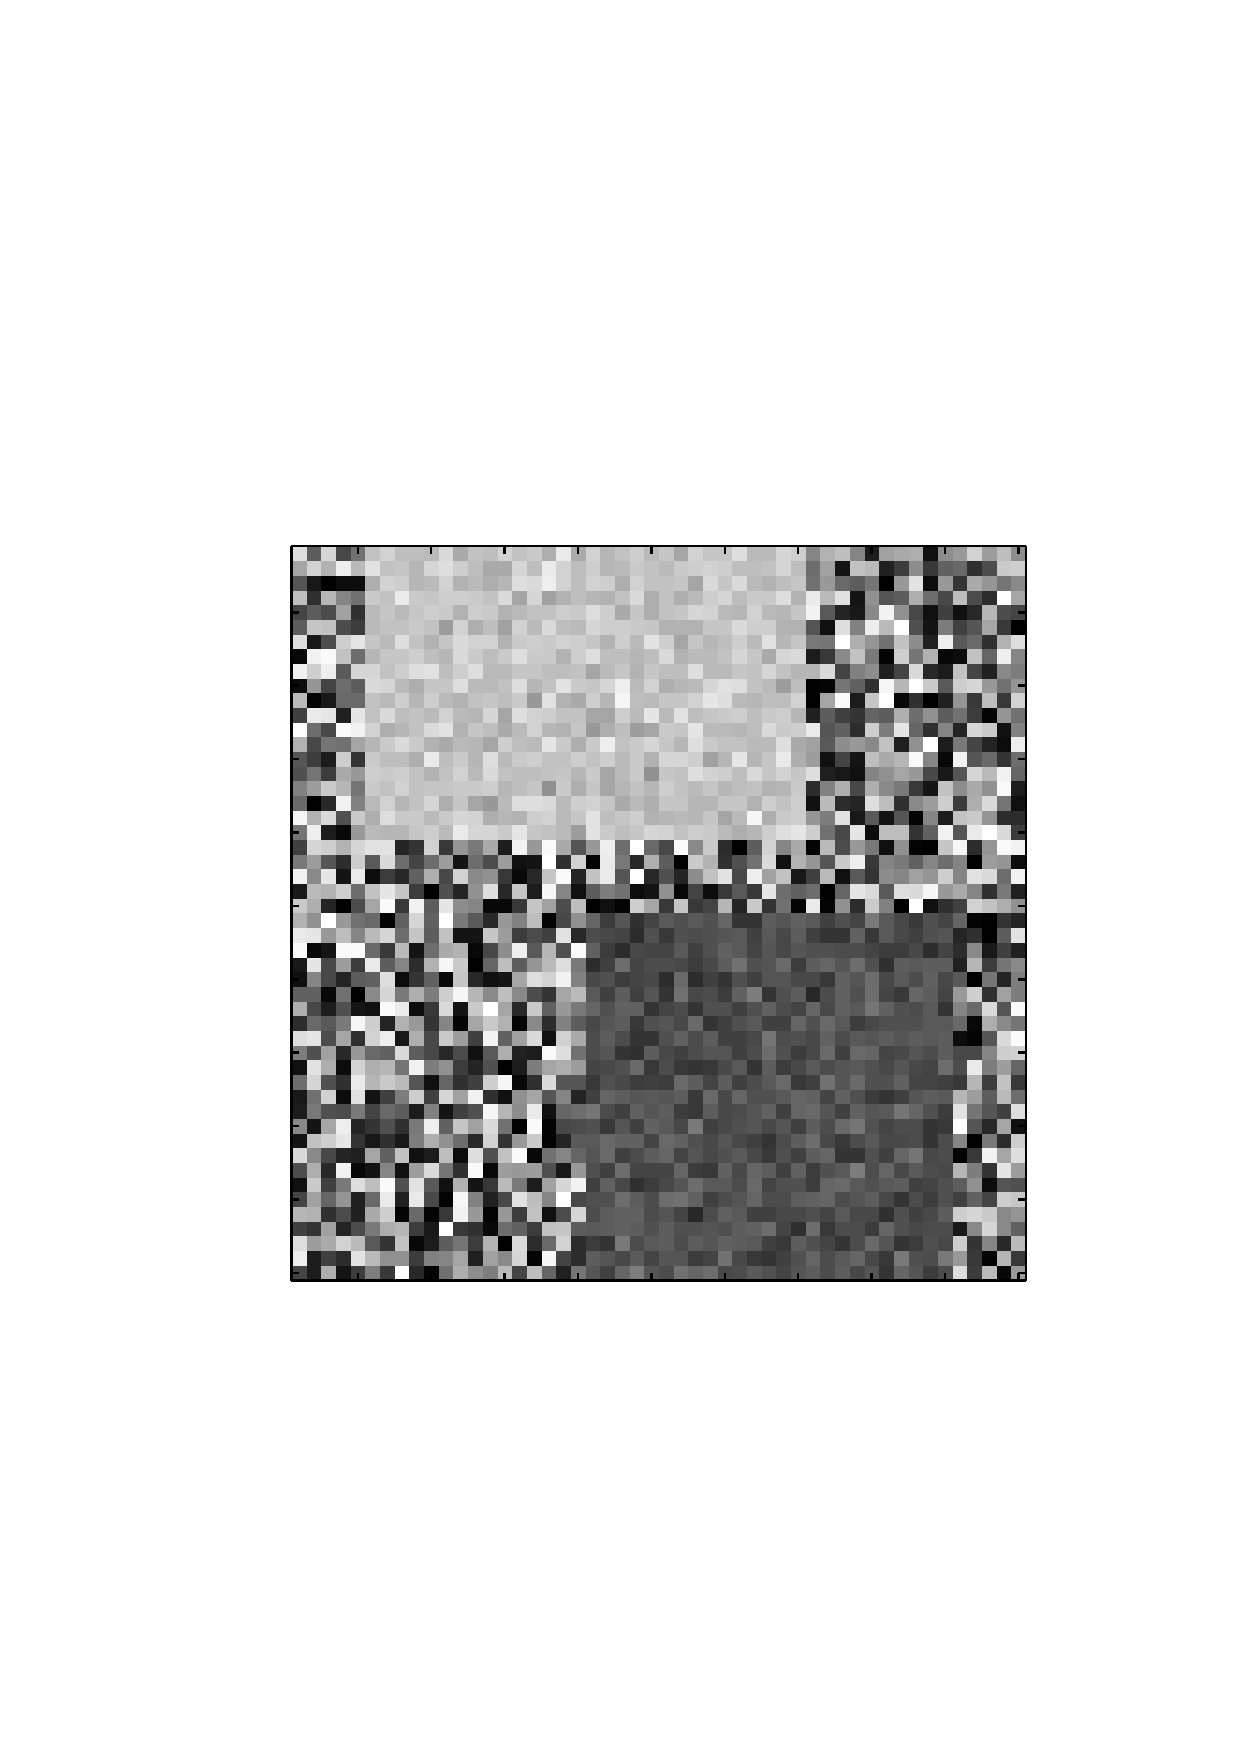
\includegraphics[width=36mm]{ori}&
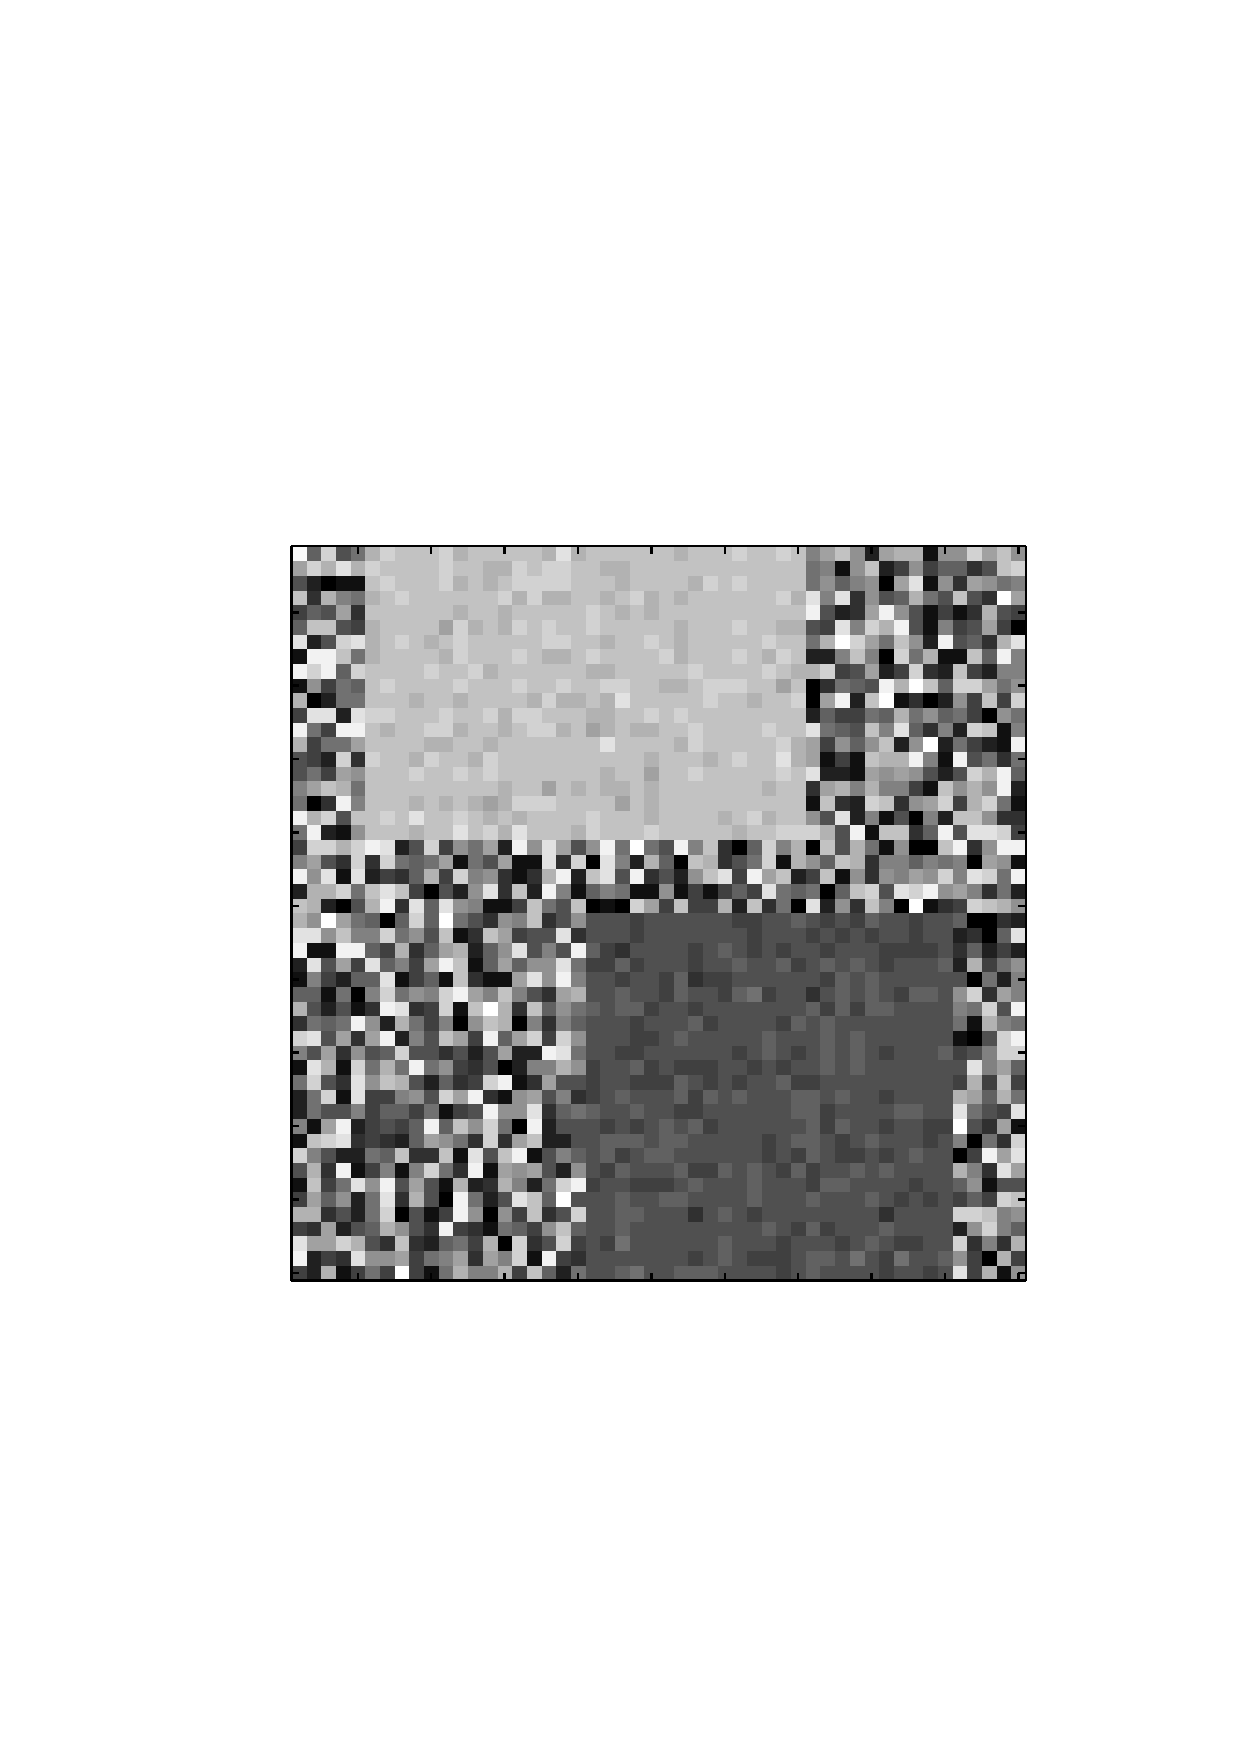
\includegraphics[width=36mm]{lp1}&
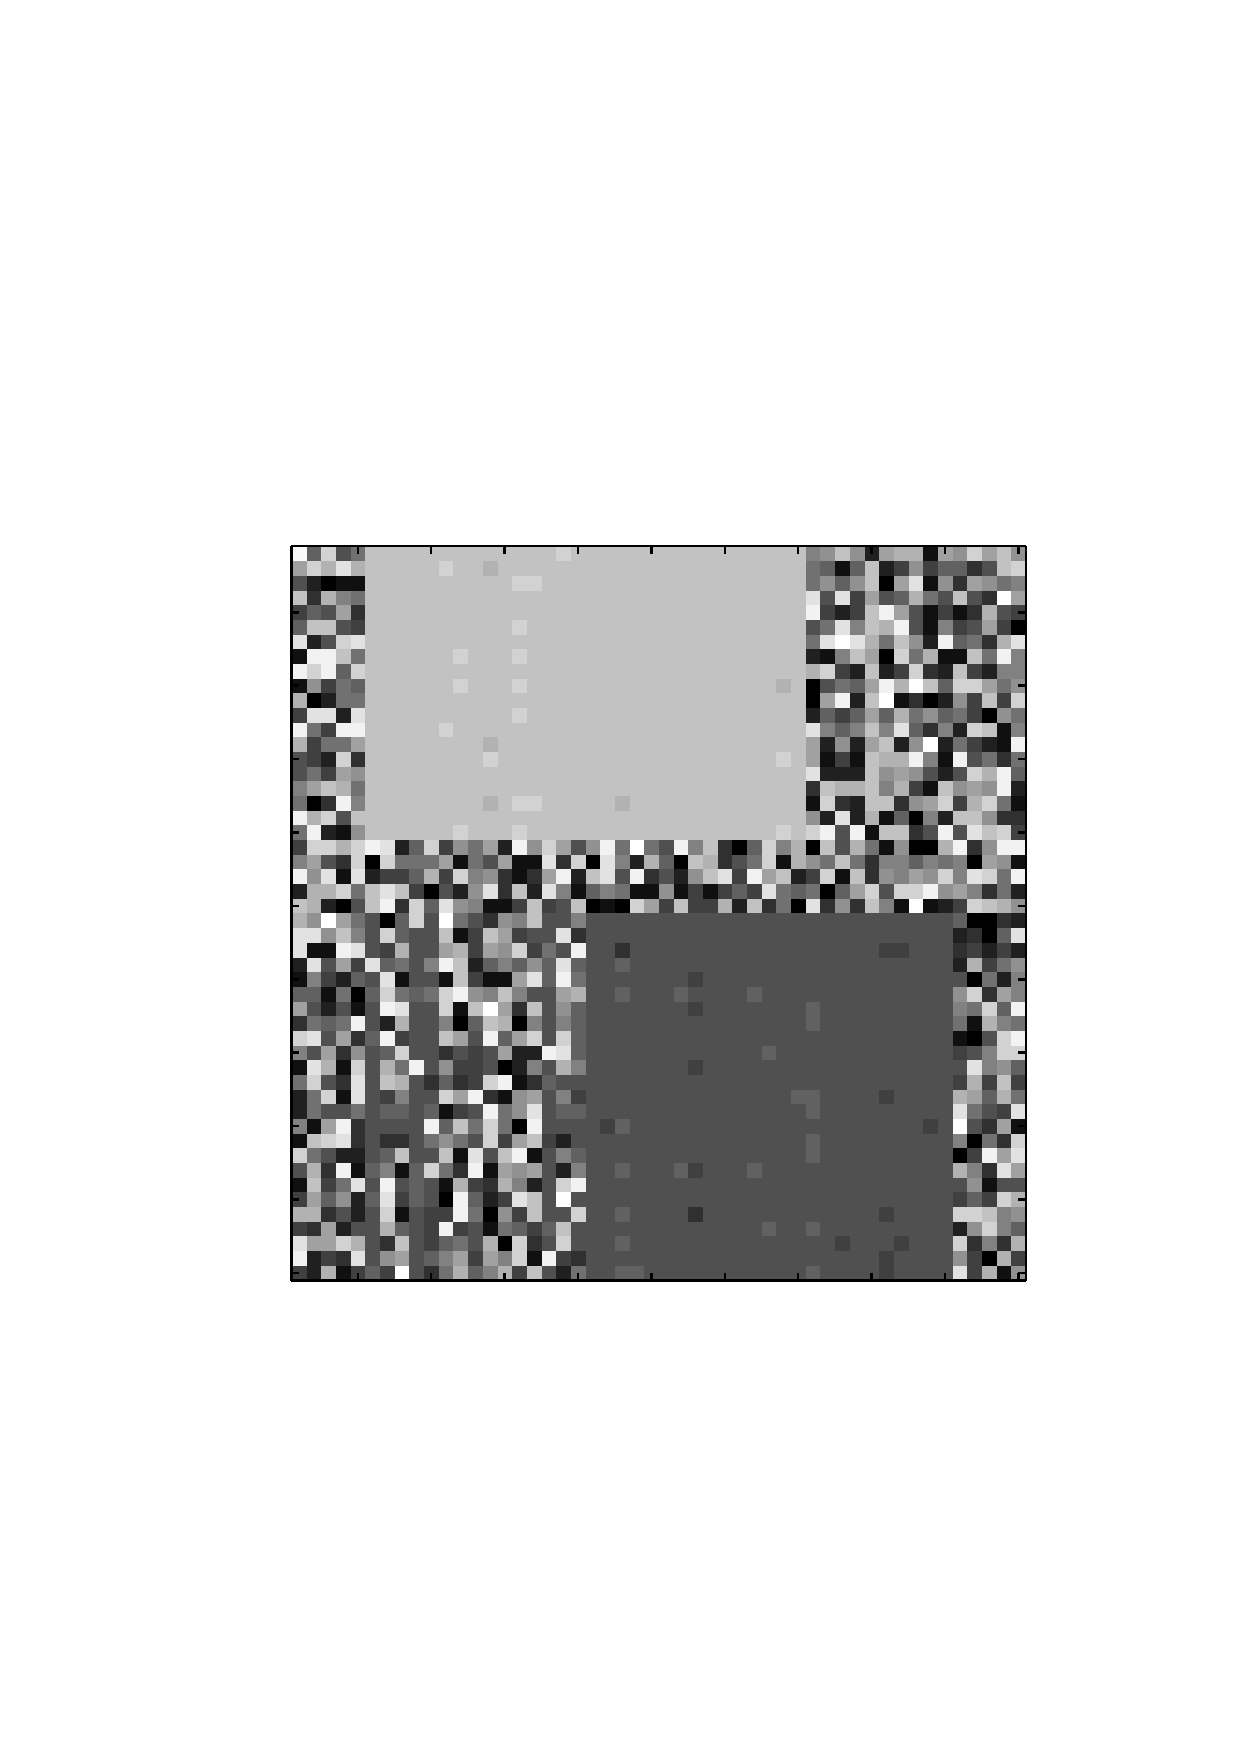
\includegraphics[width=36mm]{lp5}&
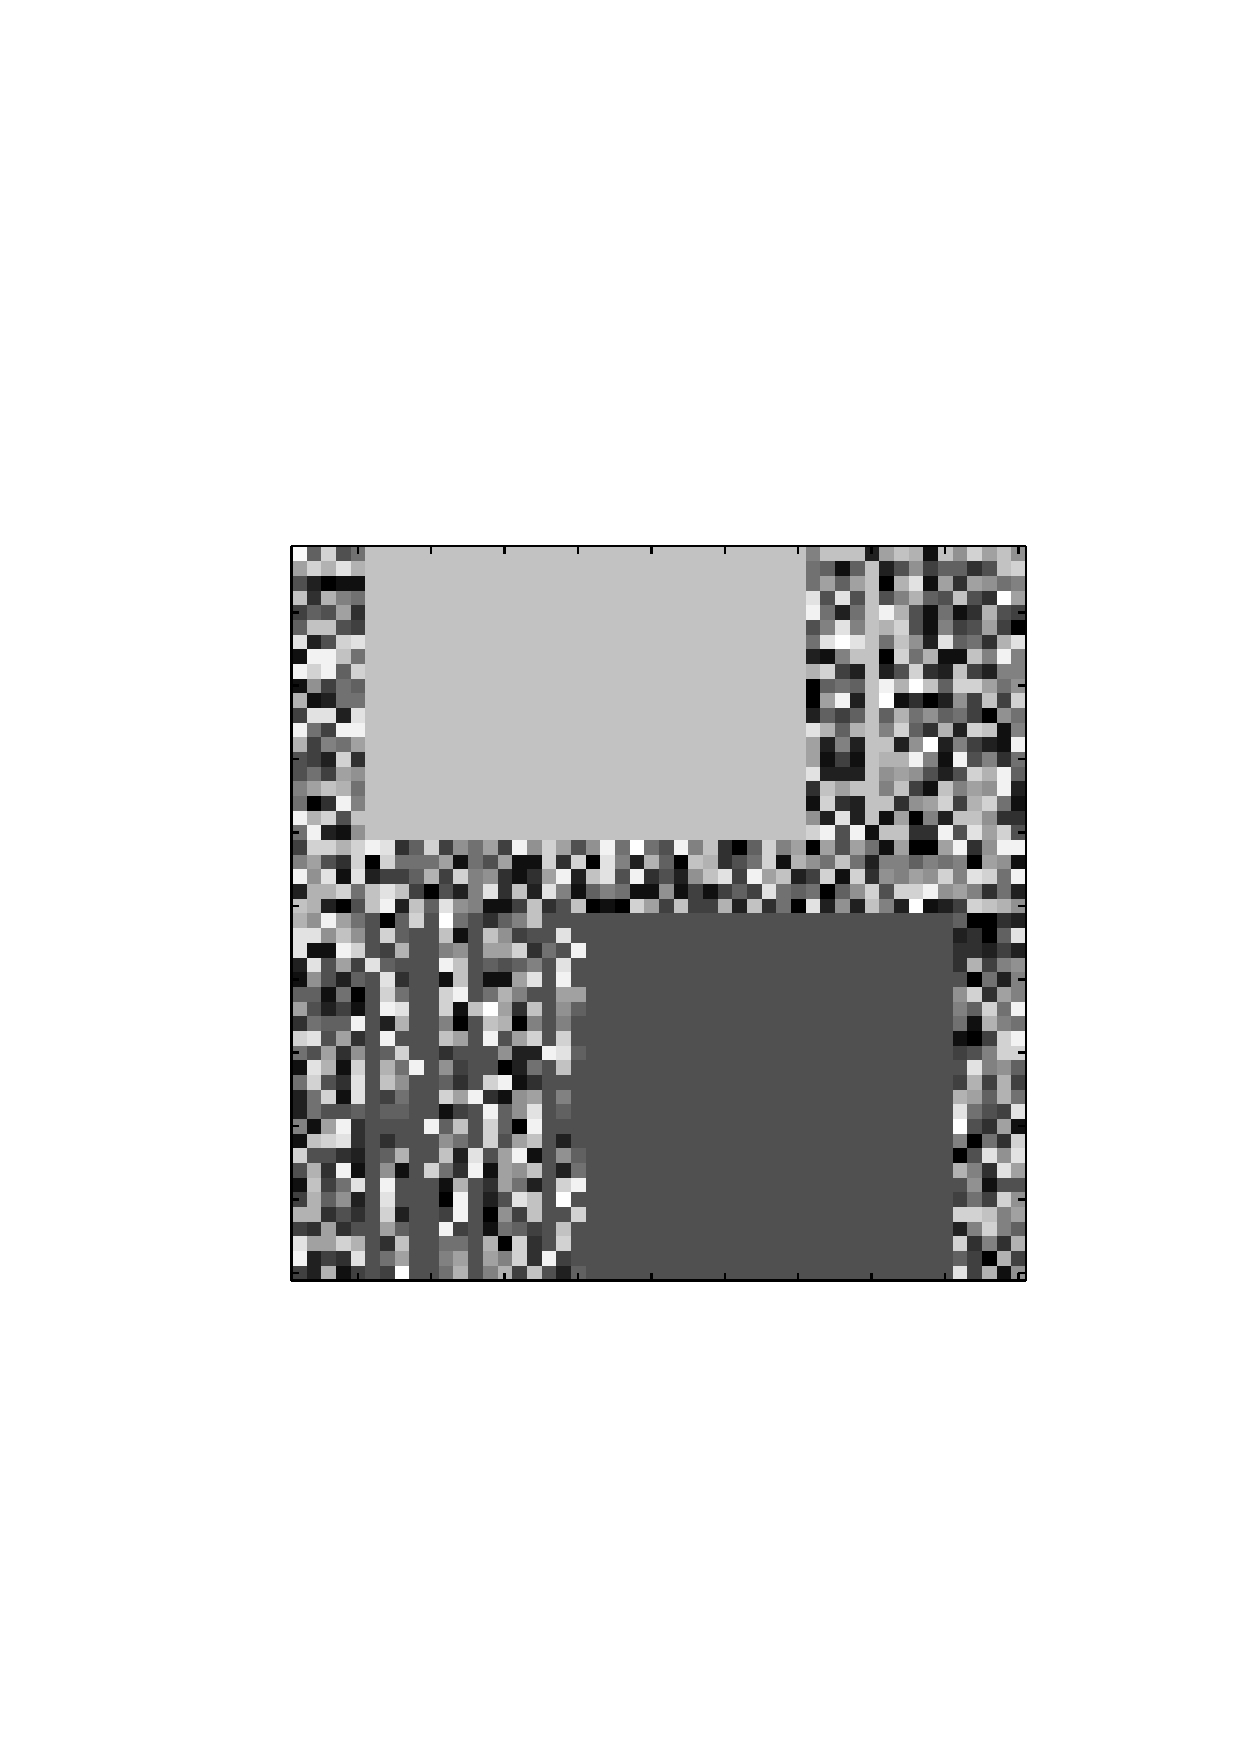
\includegraphics[width=36mm]{lp50}\\
(a) 原始矩阵 & (b) T = 1 & (c) T = 5 & (d) T = 30
\end{tabular}
\caption{\cosync算法动态双边交互过程图。 (a)原始矩阵及包含在其中的两个联合簇。(b)-(c)动态交互在的过程,可以看出联合簇中的值随着时间渐渐同步。(d)算法收敛的同步矩阵,可以看到两个嵌入的聚类簇被完美地发掘出来。}
\label{fig:simulation}
\end{figure*}

可以看出图中两个联合簇的轮廓,需要注意的是,产生这种可见“轮廓”的原因是为了可视化方便而设置的,当矩阵的行、列顺序被打乱后,联合簇将无法被肉眼识别出来,但行、列顺序并不影响\cosync算法的工作。

\vspace{2mm}
图\ref{fig:simulation}(b)-(d)展示了\cosync算法的工作流程。$T$代表双边交互模型的迭代次数,可见在$T=5$次迭代处,联合簇的轮廓就已经逐渐清晰。往后的迭代中,收敛速度逐渐变慢,直到进行到30次,程度因子的改变量小于一定阈值,停止迭代得到收敛的同步矩阵。原始的两个联合簇都被完整地挖掘出来。图\ref{RC}展示了这一过程中程度因子$r$的收敛过程。
\vspace{2mm}
\pic[htb]{程度因子随时间收敛图}{width=80mm}{RC}

从图中可以看到程度因子将收敛于$1$,且其收敛的速度初始很快,随着迭代的进行越来越缓慢,形成一个平稳的曲线。

受限于篇幅的原因,关于更多\cosync在人工数据集上的结果被置于附录中。从这些实验中我们可以得出结论,\cosync算法对于原始矩阵中嵌入的少量大尺寸联合簇的挖掘结果表现良好,受动态同步的思想驱动,嵌入在数据集中的联合簇都被自然地挖掘了出来,且对参数的上下浮动的敏感性较低,具有不错的鲁棒性。但是若在数据集中嵌入的联合簇的分布复杂,且尺寸小数量多的情况下,则受限于相似性度量难以有效发挥作用,不能很好地同步在一起。

\subsection{\cosync与其他算法的性能比较}
\label{subsec:compare}
为了证明我们的算法相对于与其他算法的优势,说明\cosync算法能挖掘出任意排列方式的联合簇,我们设计了两个代表性的$(1000\times1000)$的中大型数据矩阵。其中一个矩阵中的联合簇将以棋盘(checkboard)的方式分布,如图\ref{fig:yiqi}(a)所示;而另一个矩阵中的联合簇位置分布任意,如图\ref{fig:yiqi}(c)所示。图中矩阵里嵌入的颜色深浅不一的子矩阵从均值不一的高斯分布$N(\mu,\sigma)$中采样得到。为了消除行、列的排序对算法性能的影响,图\ref{fig:yiqi}(b)和(d)是棋盘分布矩阵和随机分布矩阵行列顺序打散后的结果。所有的实验都将在乱序上的矩阵上进行。

接着我们将分别在这两个数据矩阵上,用\cosync,ITCC,MSSRCC,Spectral Clustering,Plaid进行测试。国际上很多主流算法由于自身局限性,对数据矩阵有较强的假设:联合簇的分布为棋盘式的,比如本次进行试验的ITCC,MSSRCC和Spectral CLustering算法。在这样的假设下,这些算法将分别对行、列空间进行聚类,最后把同一个簇的行列集合放到一起形成子矩阵。此外除\cosync外的四种算法都需要指定双边聚类的行、列各自划分的数目,相当于一个先验参数。下面是两个数据集分别的实验结果:

\vspace{4mm}
\tabcolsep=2pt
\begin{figure*}[!htb]
\centering
\begin{tabular}{cccc}
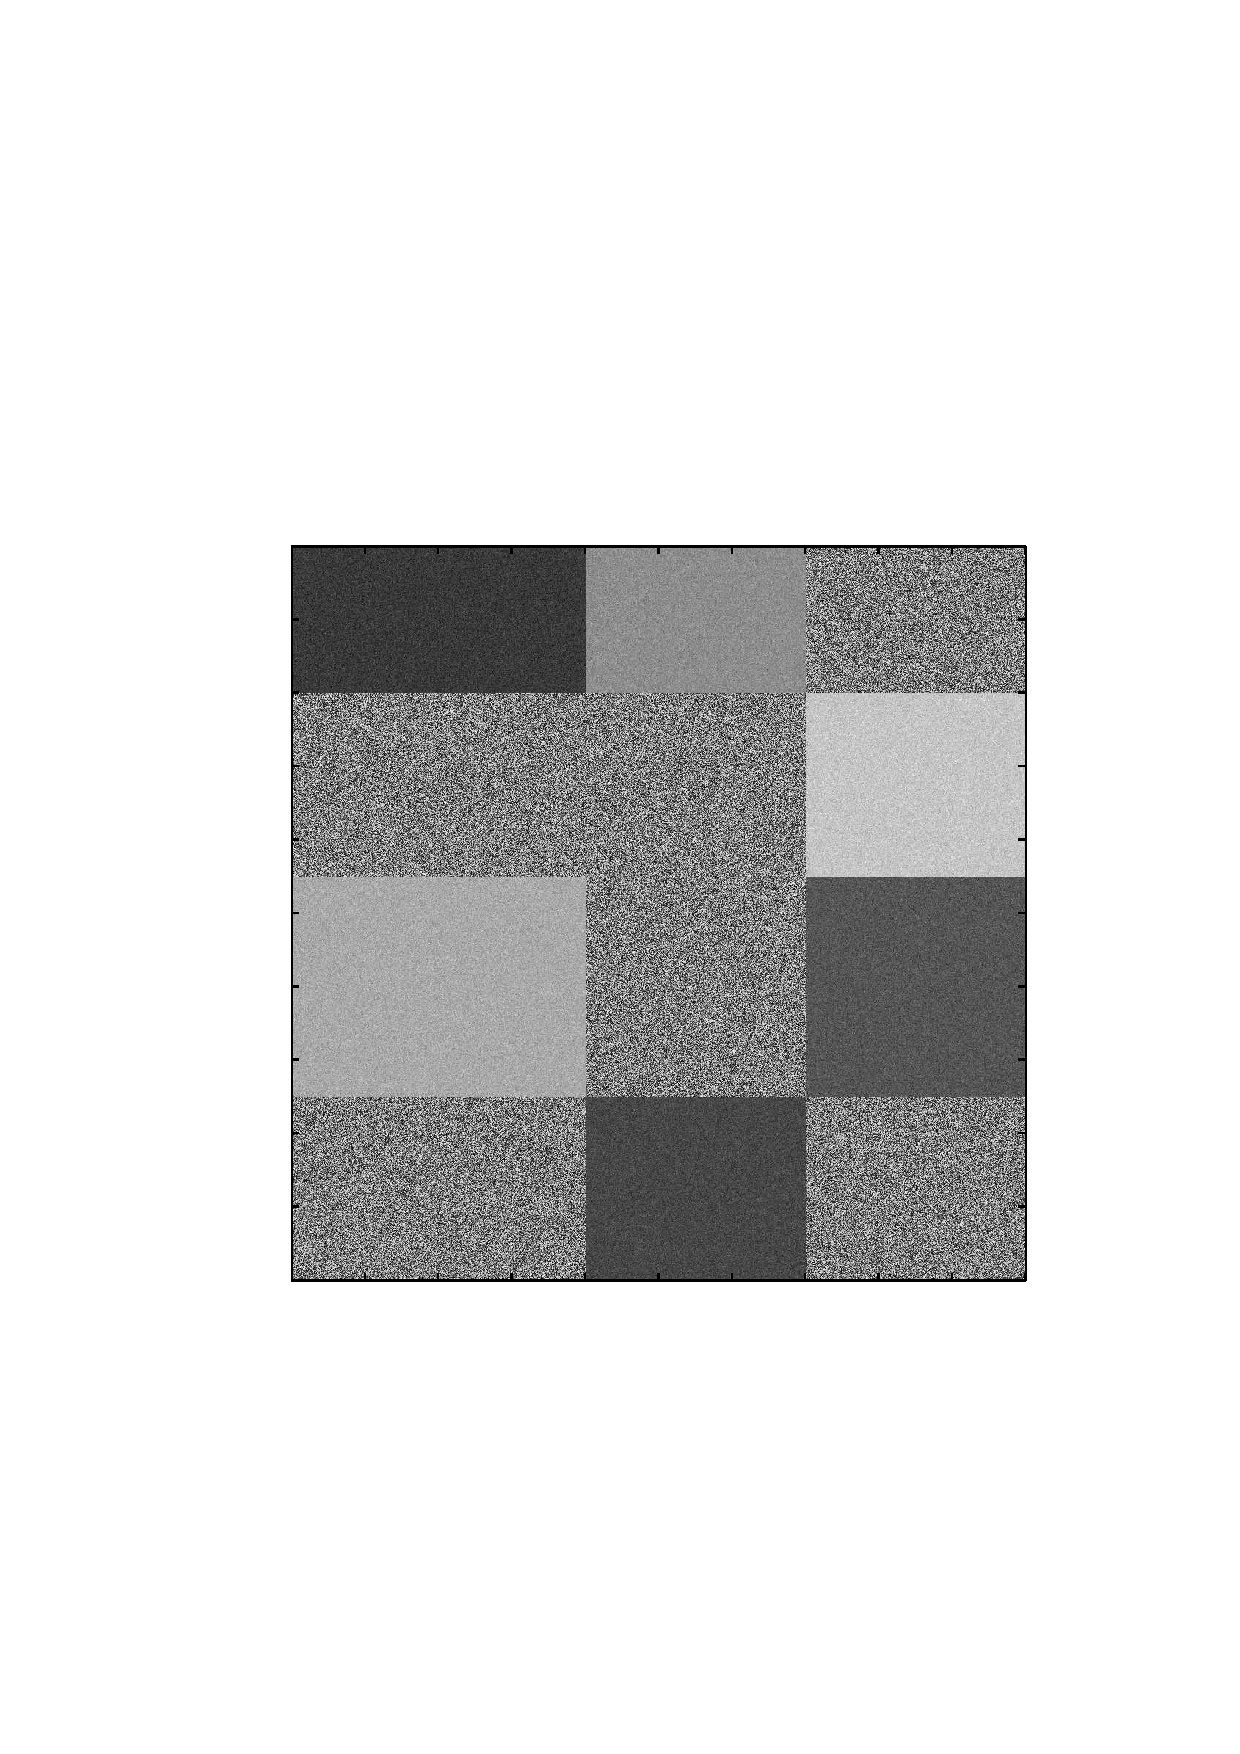
\includegraphics[width=36mm]{O1}&
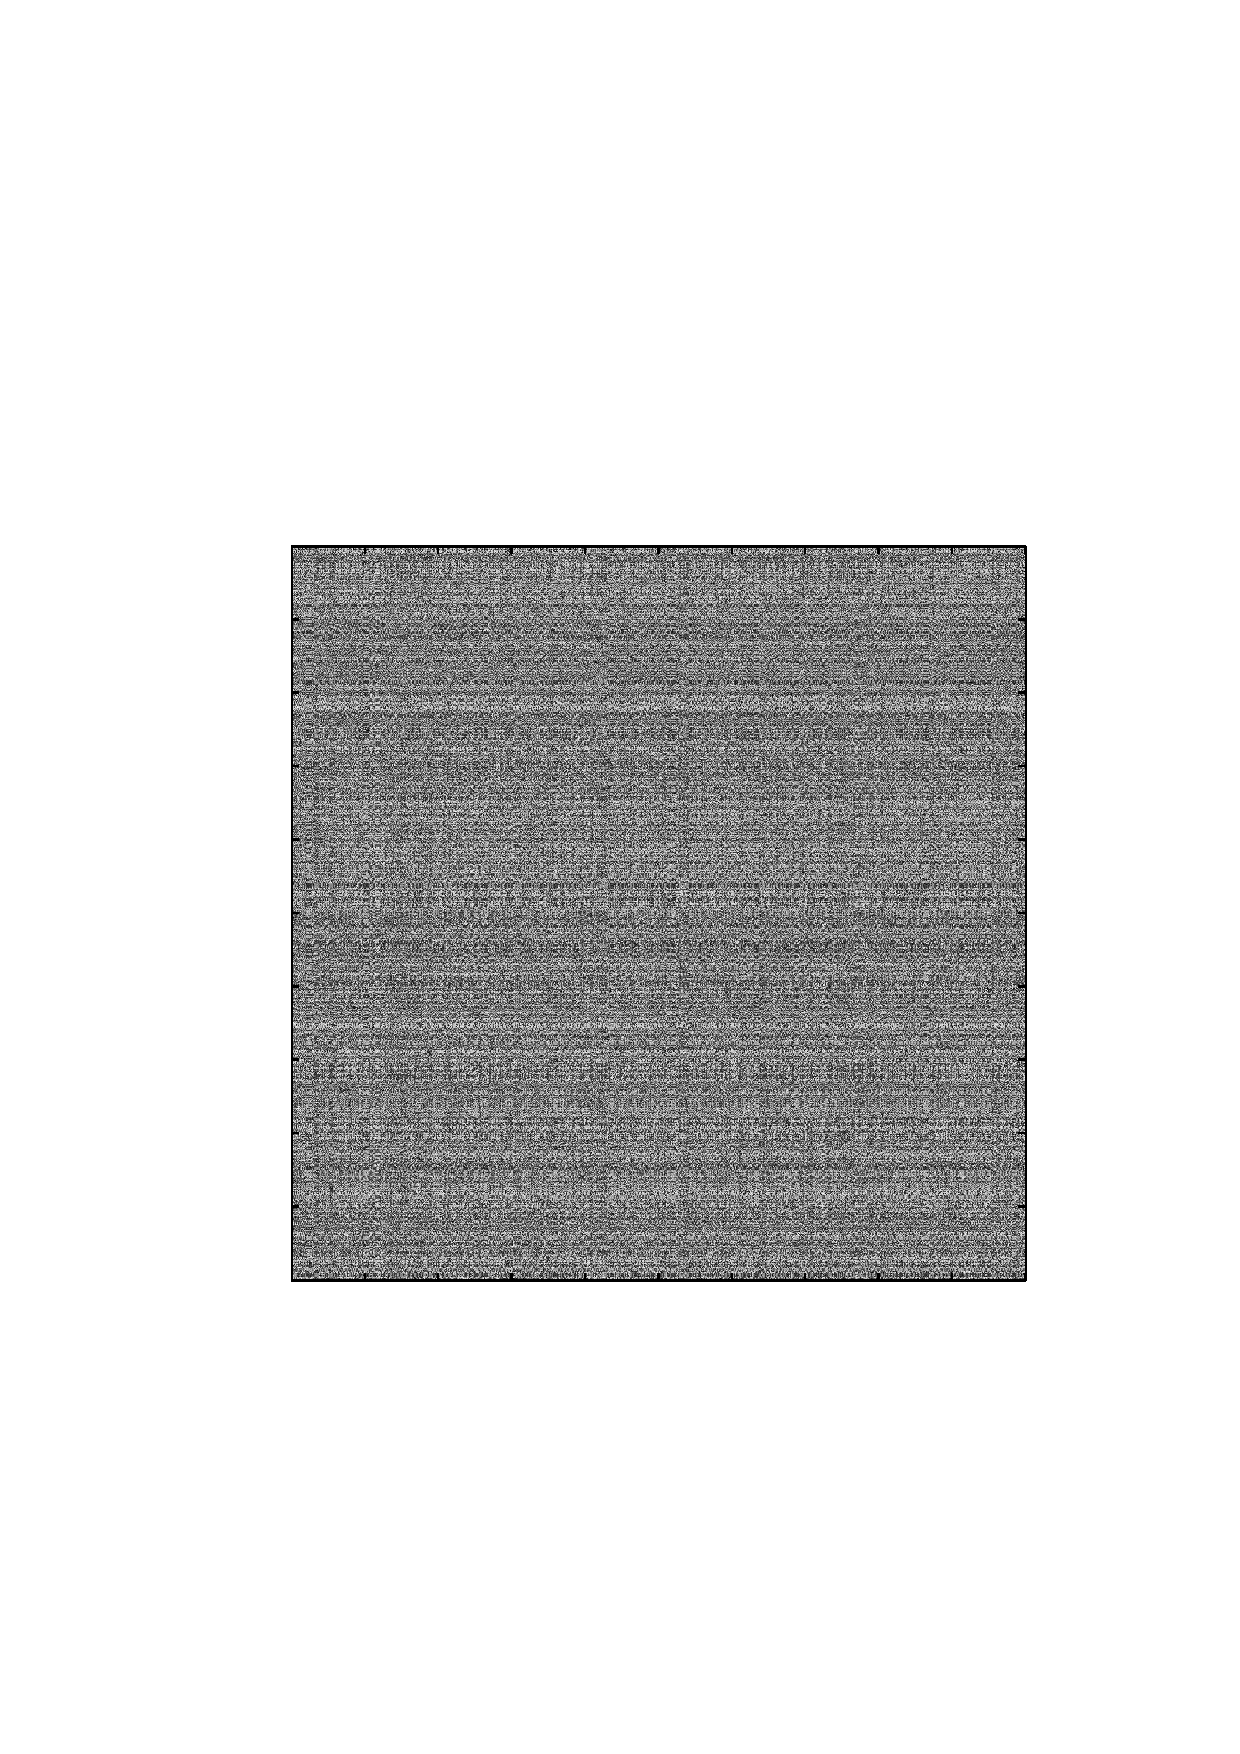
\includegraphics[width=36mm]{S1}&
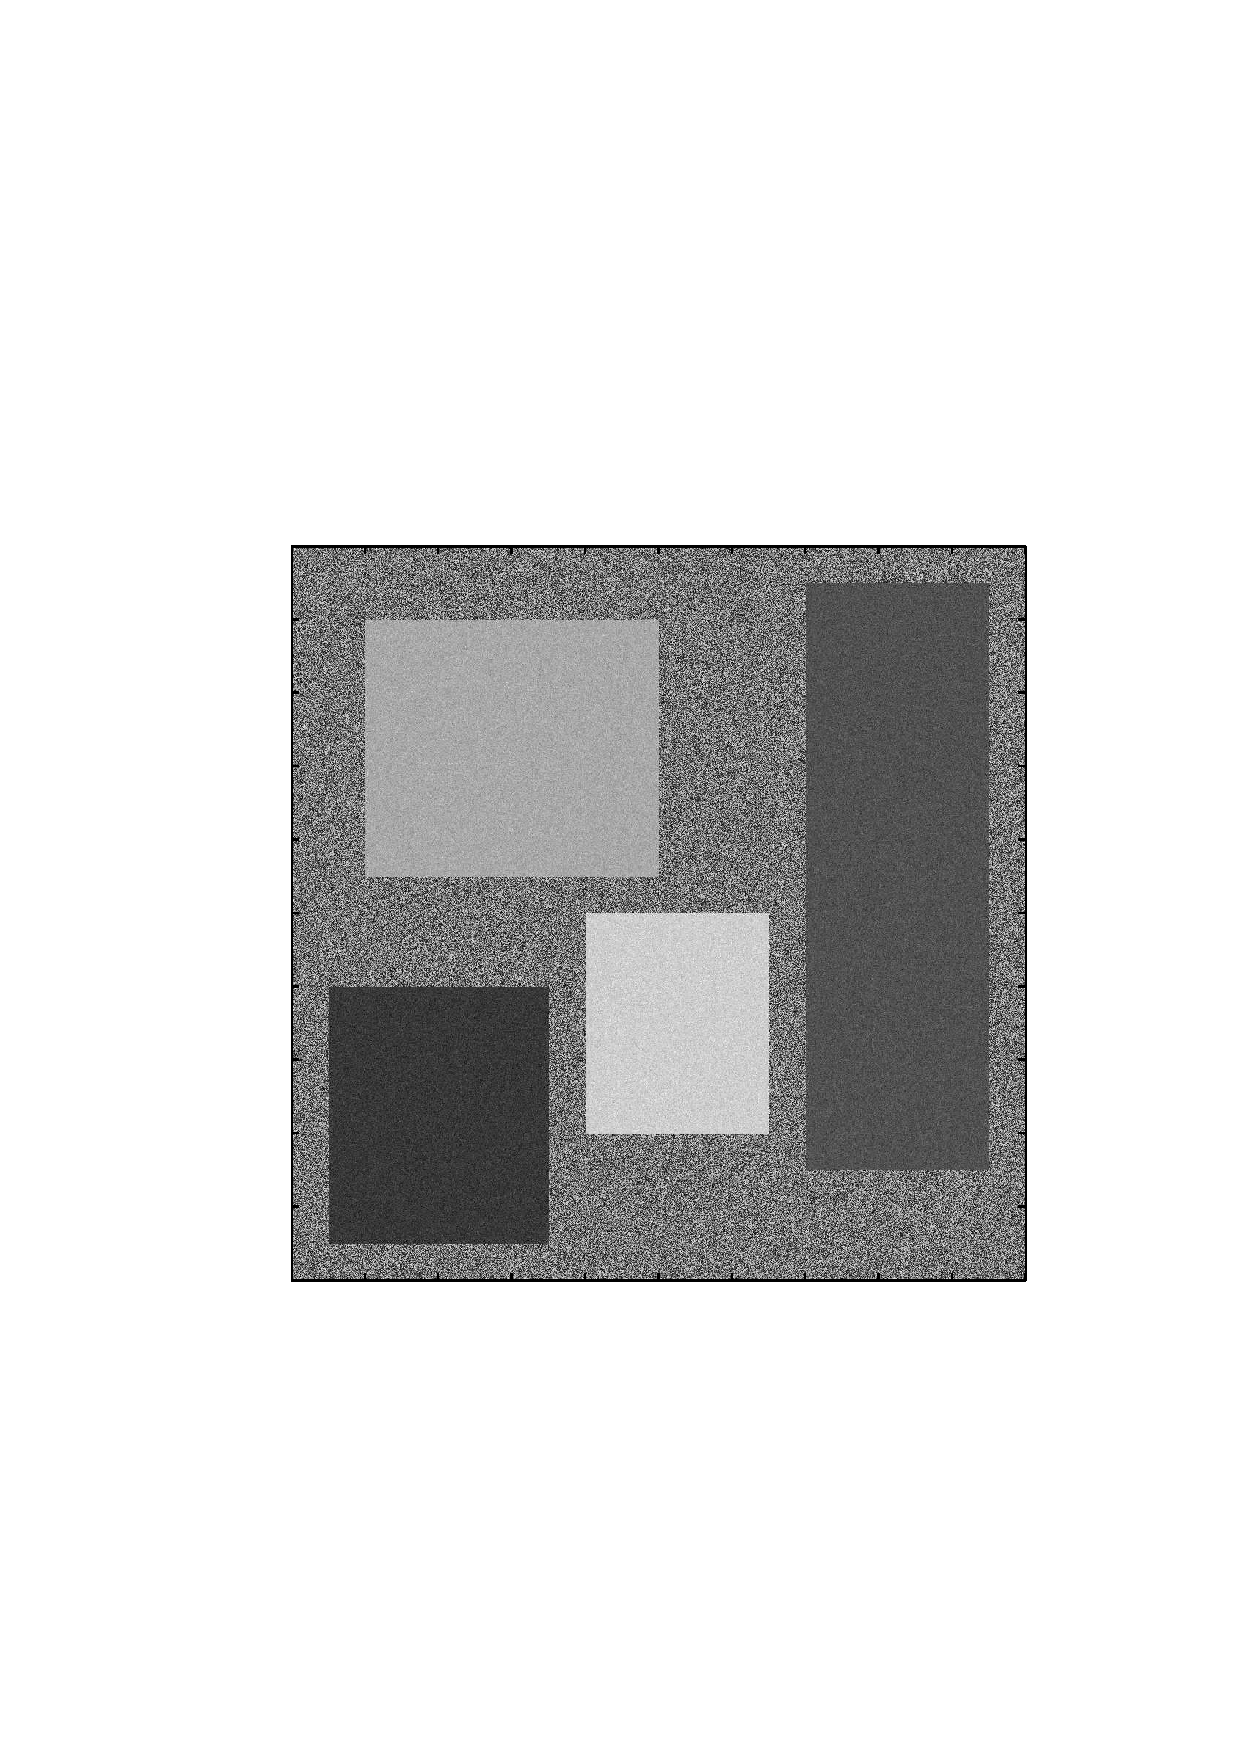
\includegraphics[width=36mm]{O2}&
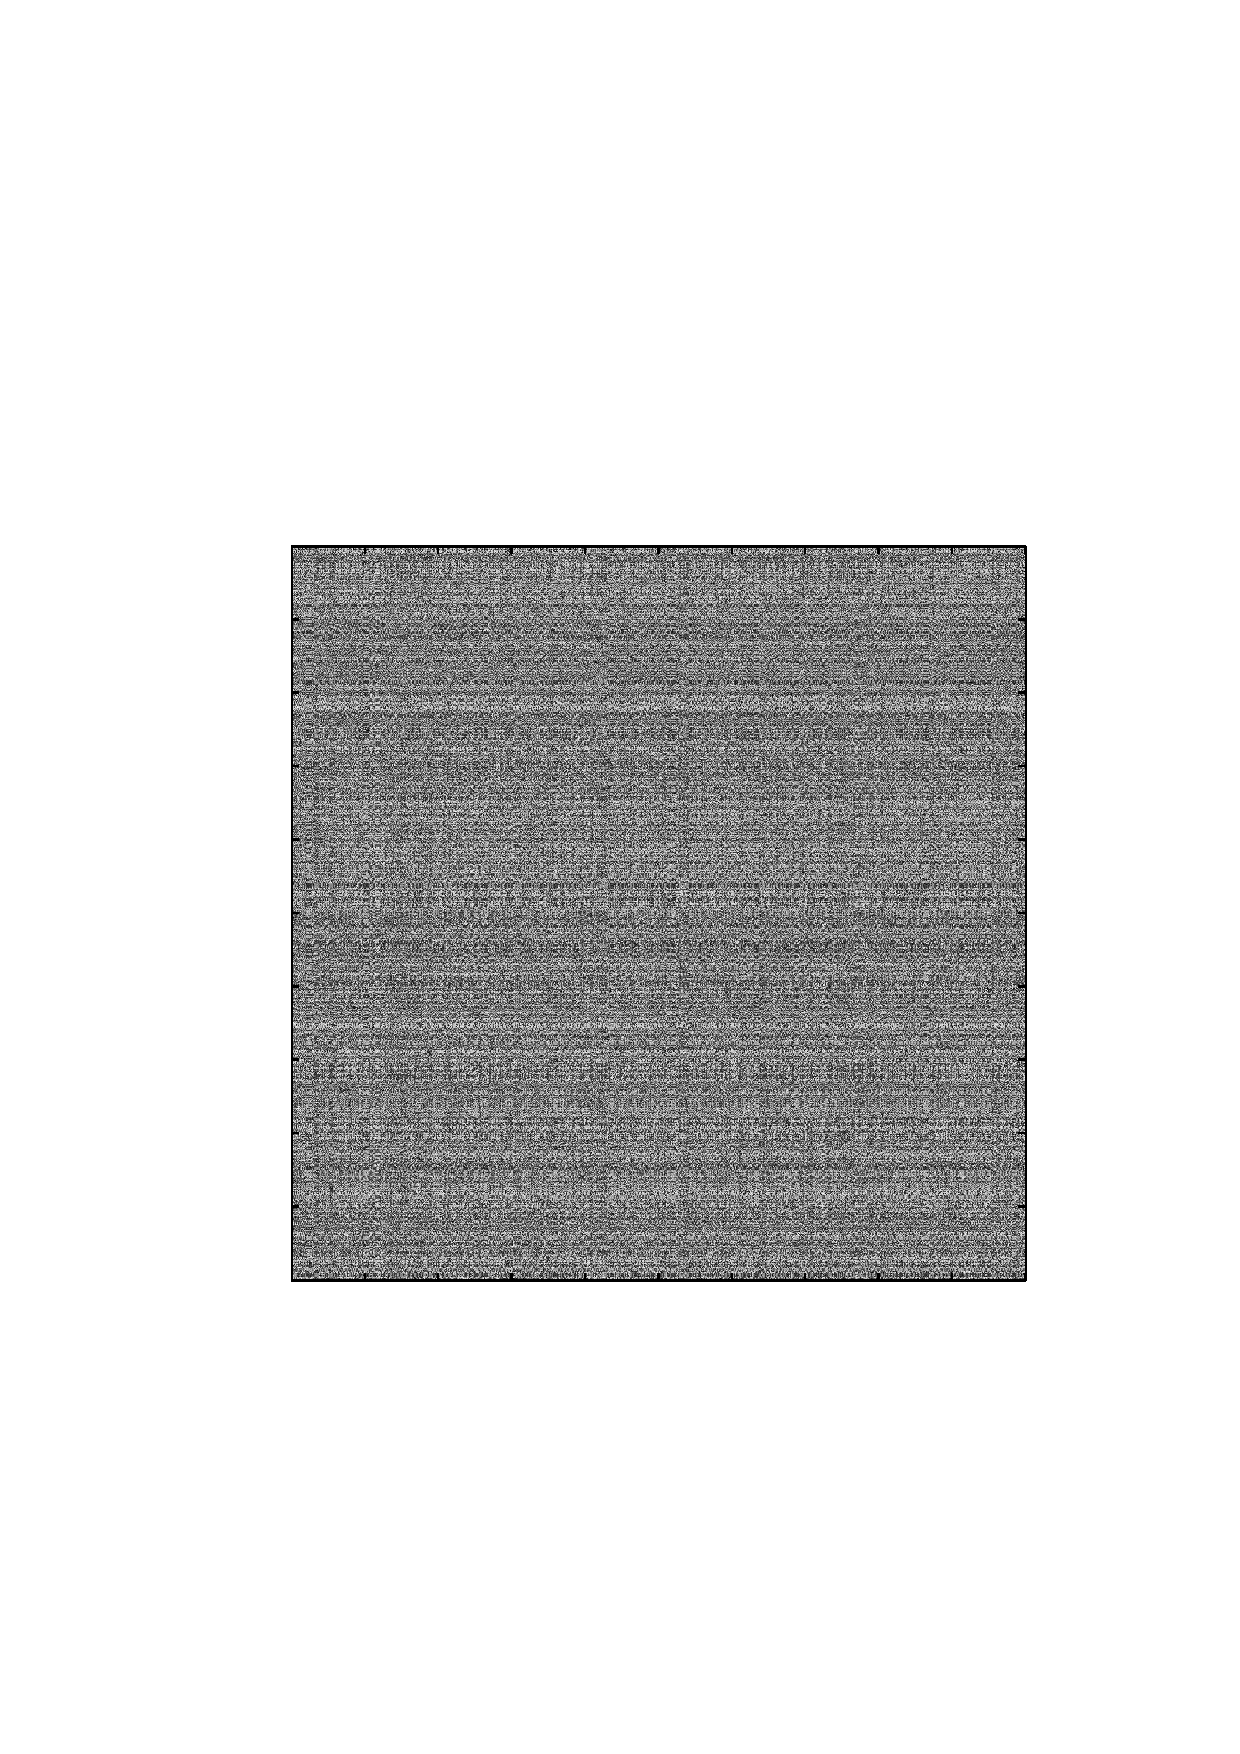
\includegraphics[width=36mm]{S1}\\
(a)棋盘分布矩阵  & (b)棋盘分布行列打散 &(c)随机分布 &(d)随机分布行列打散
\end{tabular}
\caption{棋盘分布矩阵及行列顺序打散矩阵图}
\label{fig:yiqi}
\end{figure*}


\tabcolsep=1pt
\begin{figure*}[!p]
\centering
\begin{tabular}{ccc}
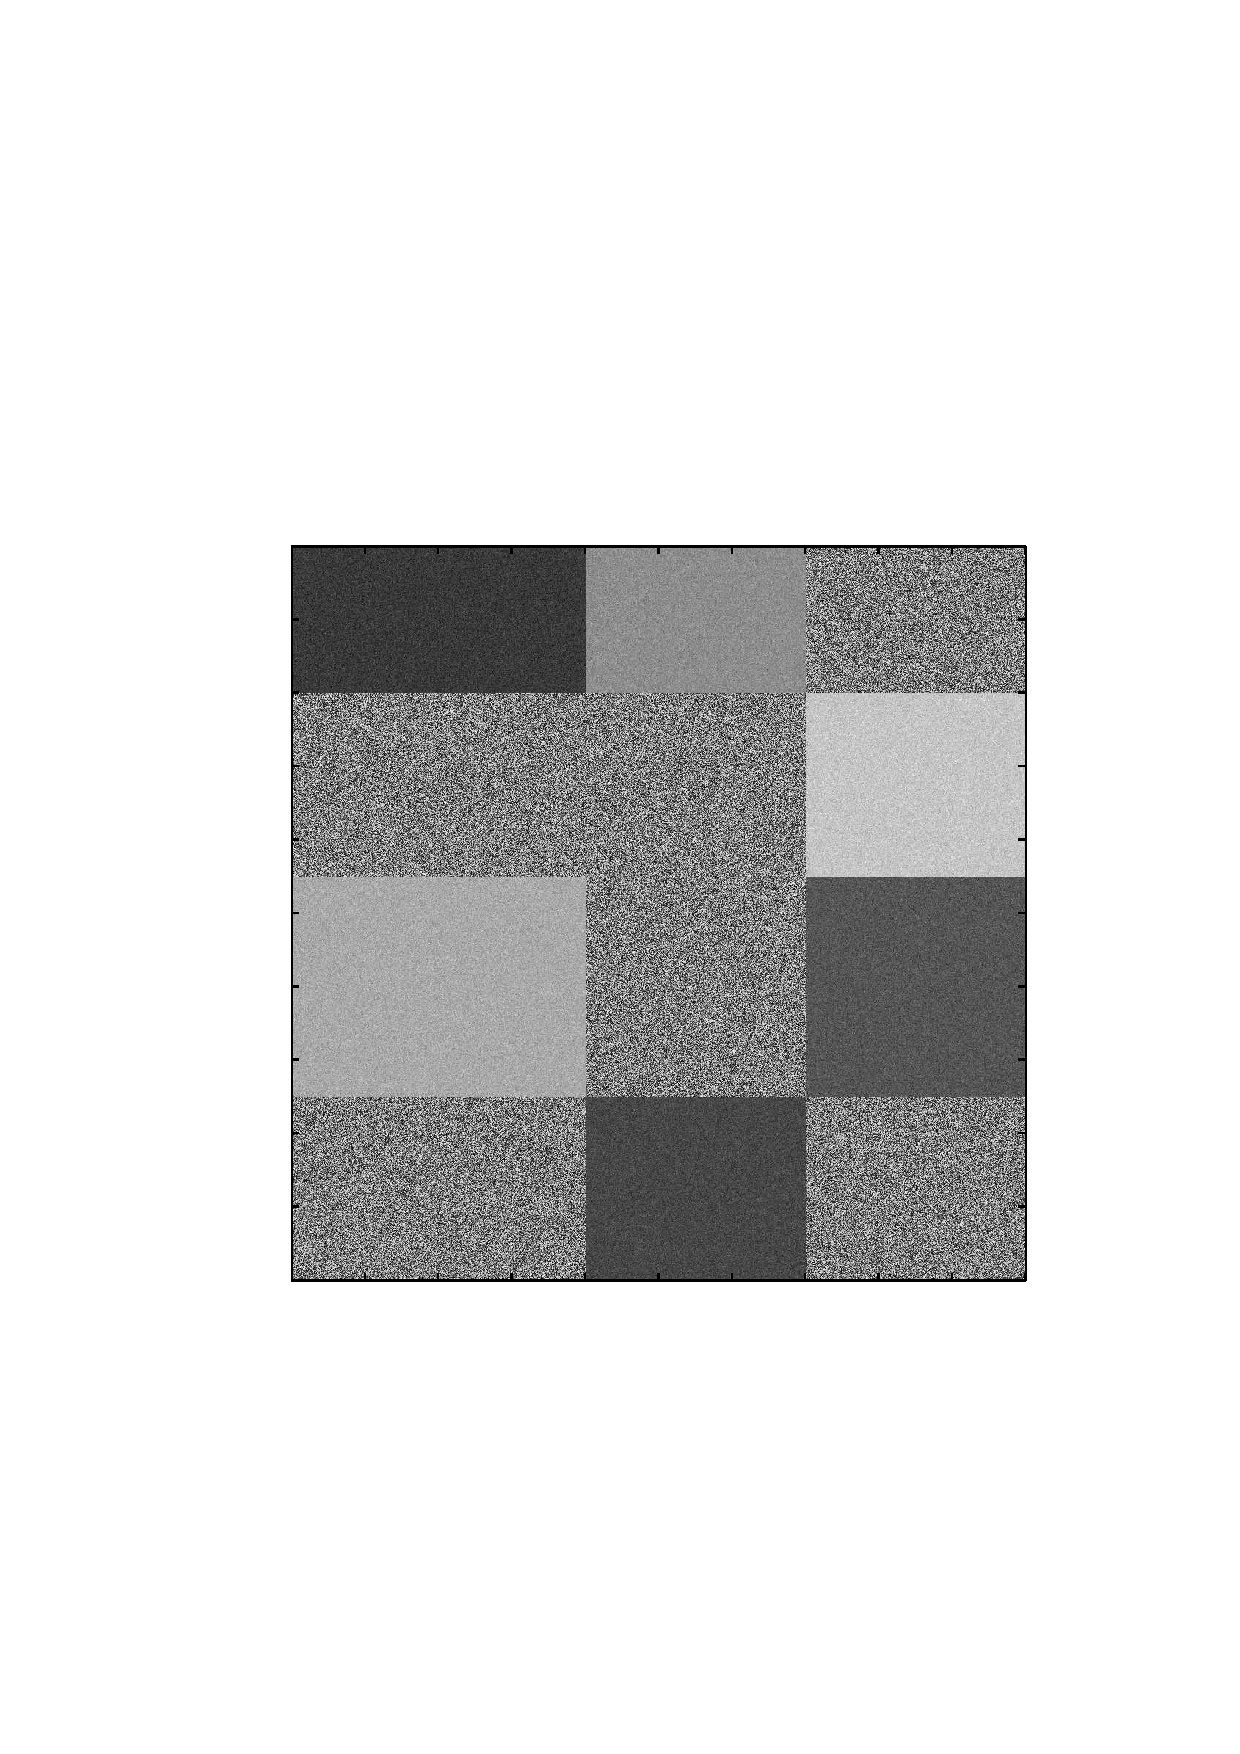
\includegraphics[width=45mm]{O1}&
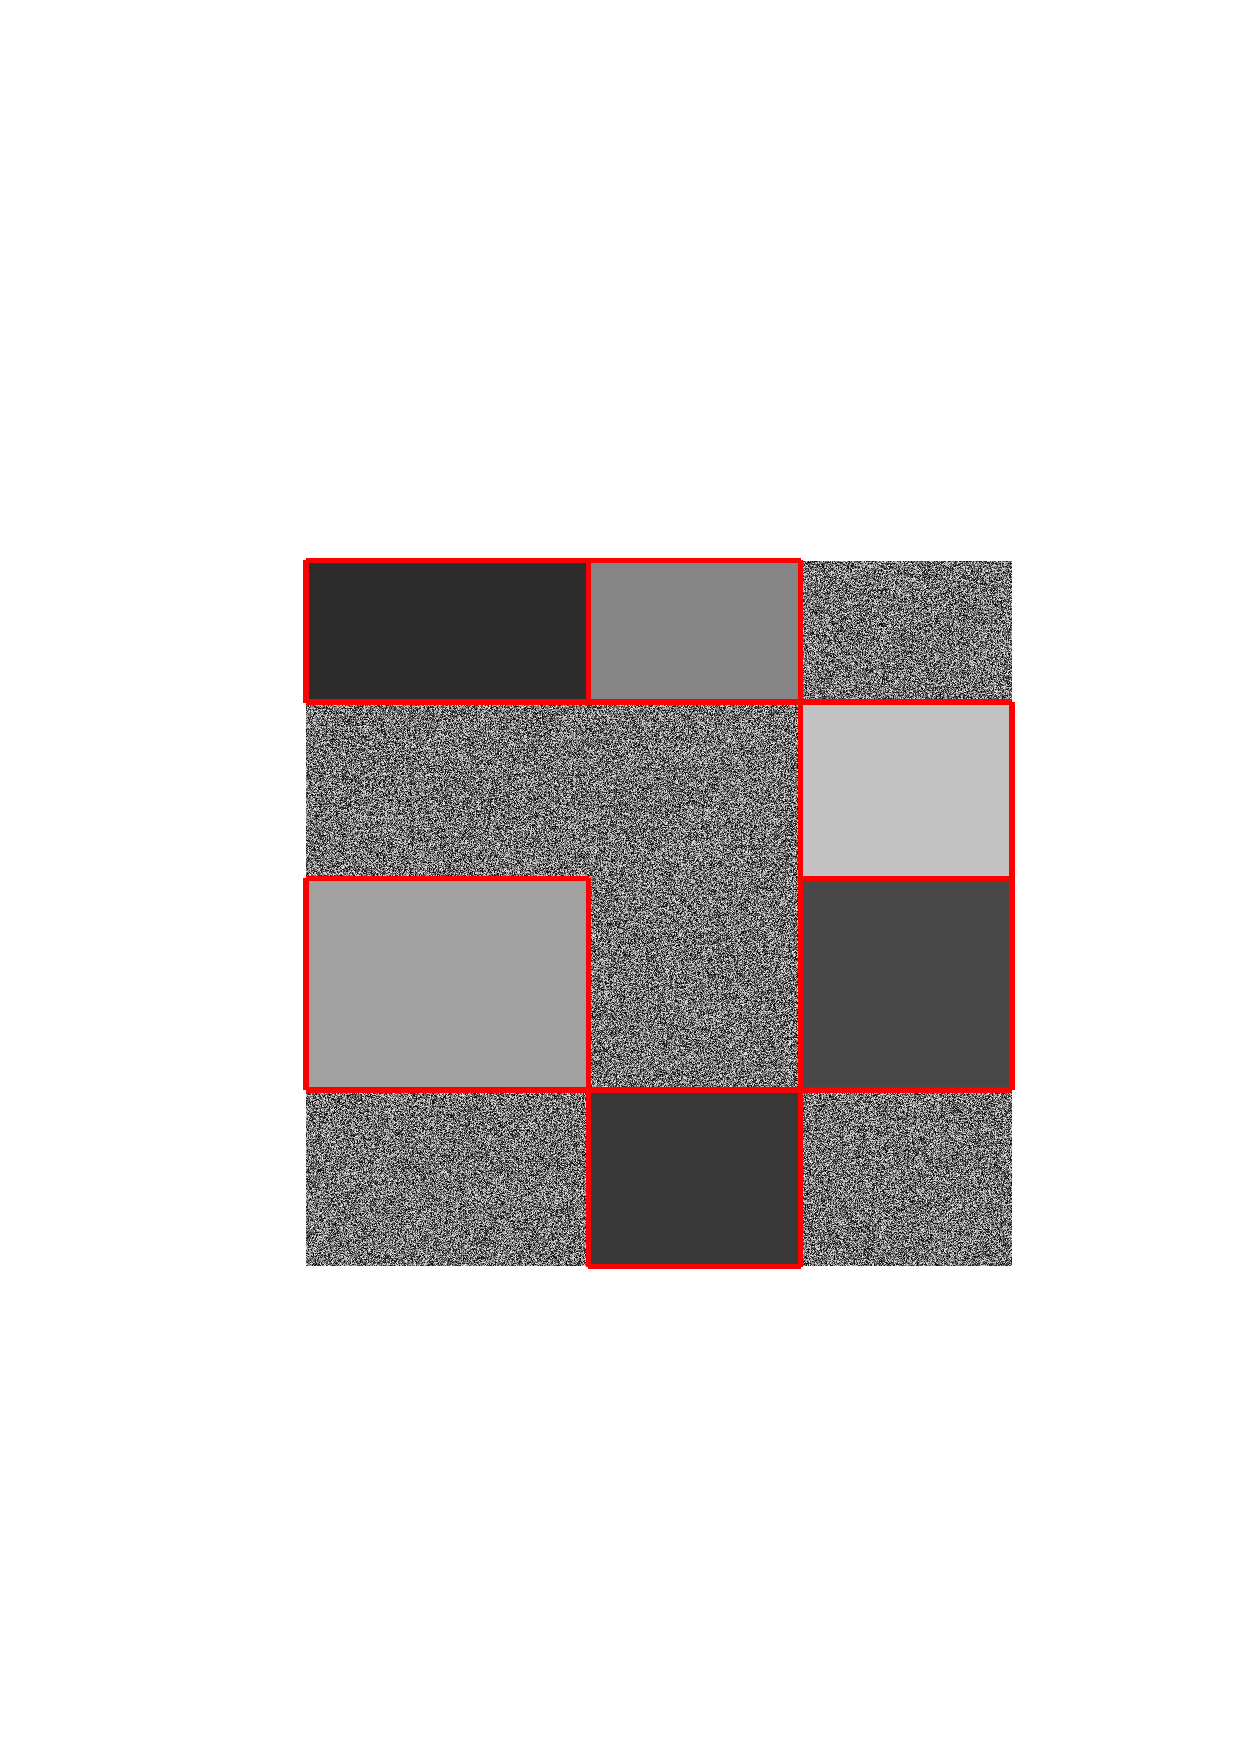
\includegraphics[width=45mm]{syn1R}&
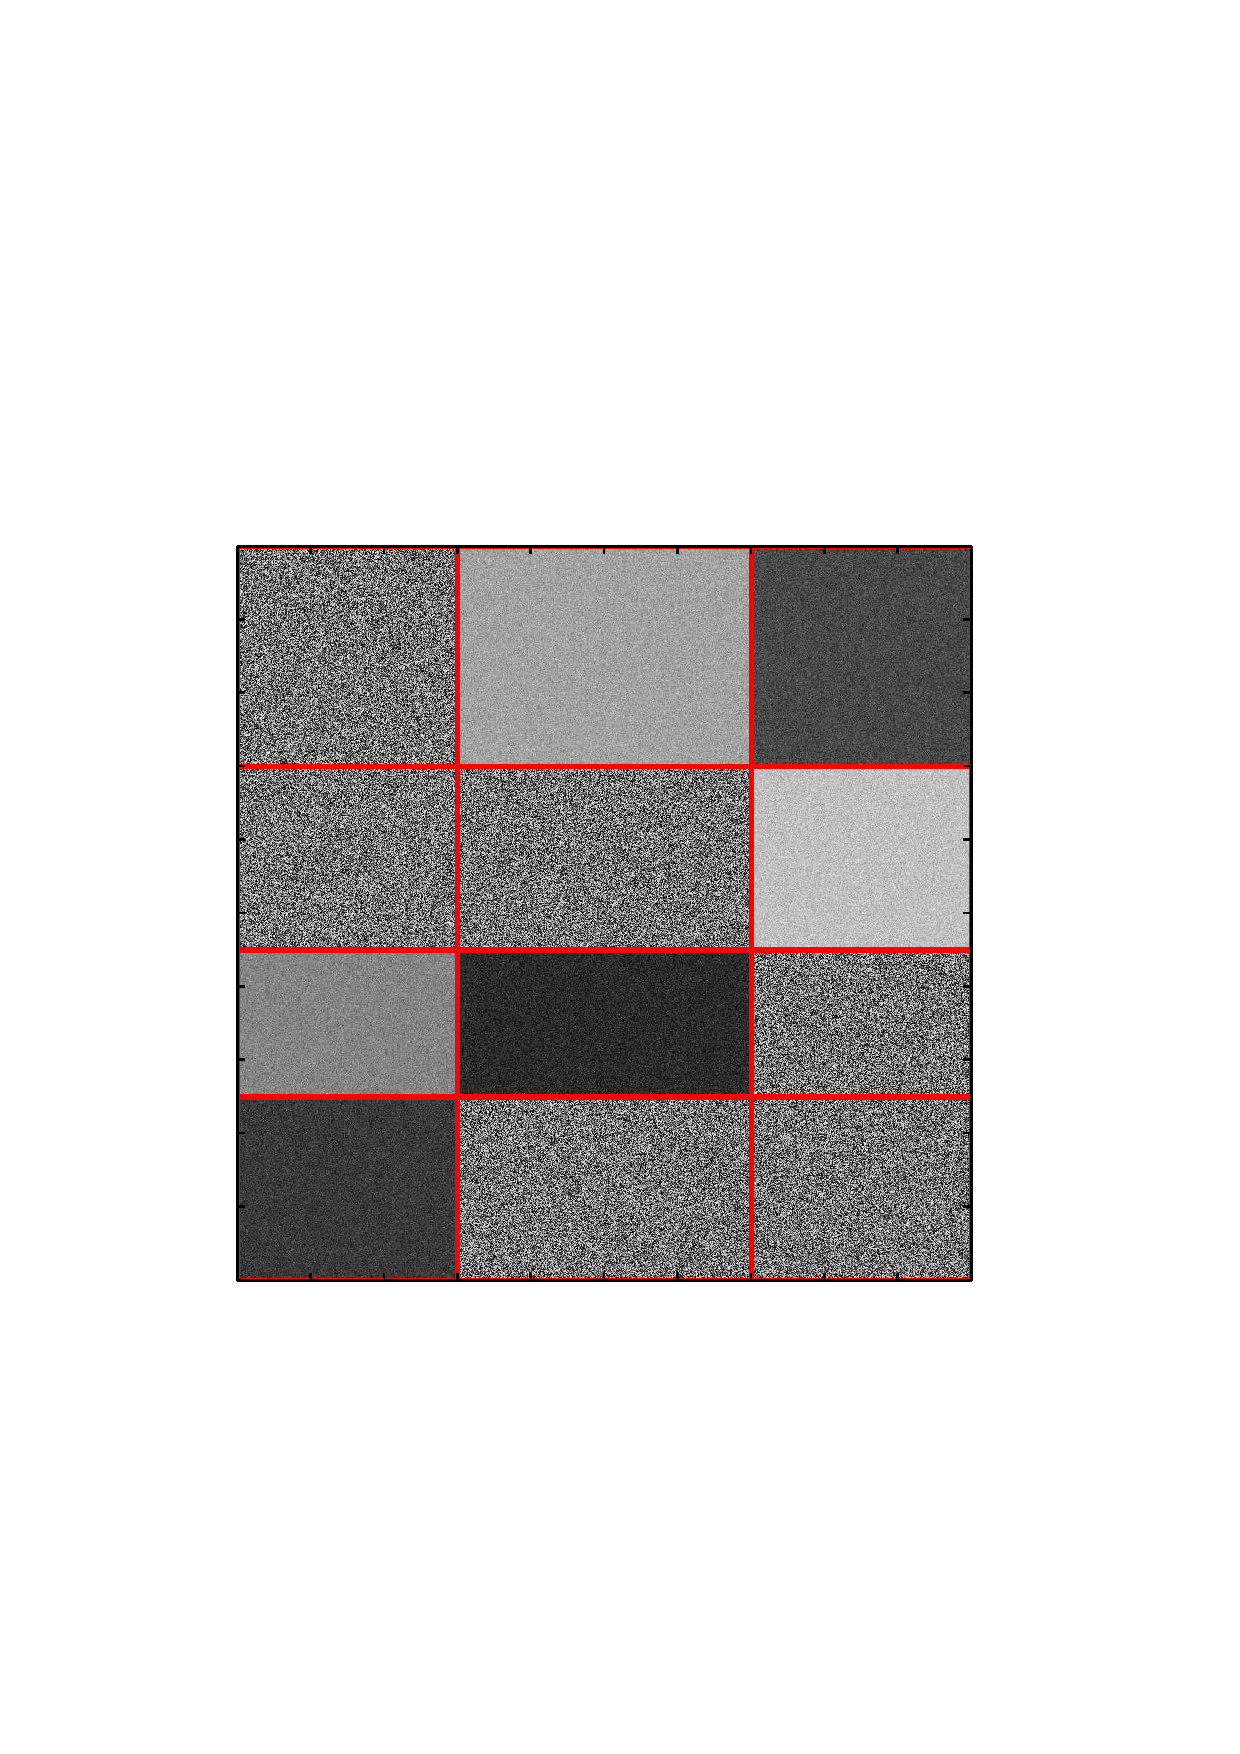
\includegraphics[width=45mm]{inf1}\\
(a) 棋盘分布矩阵  & (b) CoSync &  (c) ITCC\\
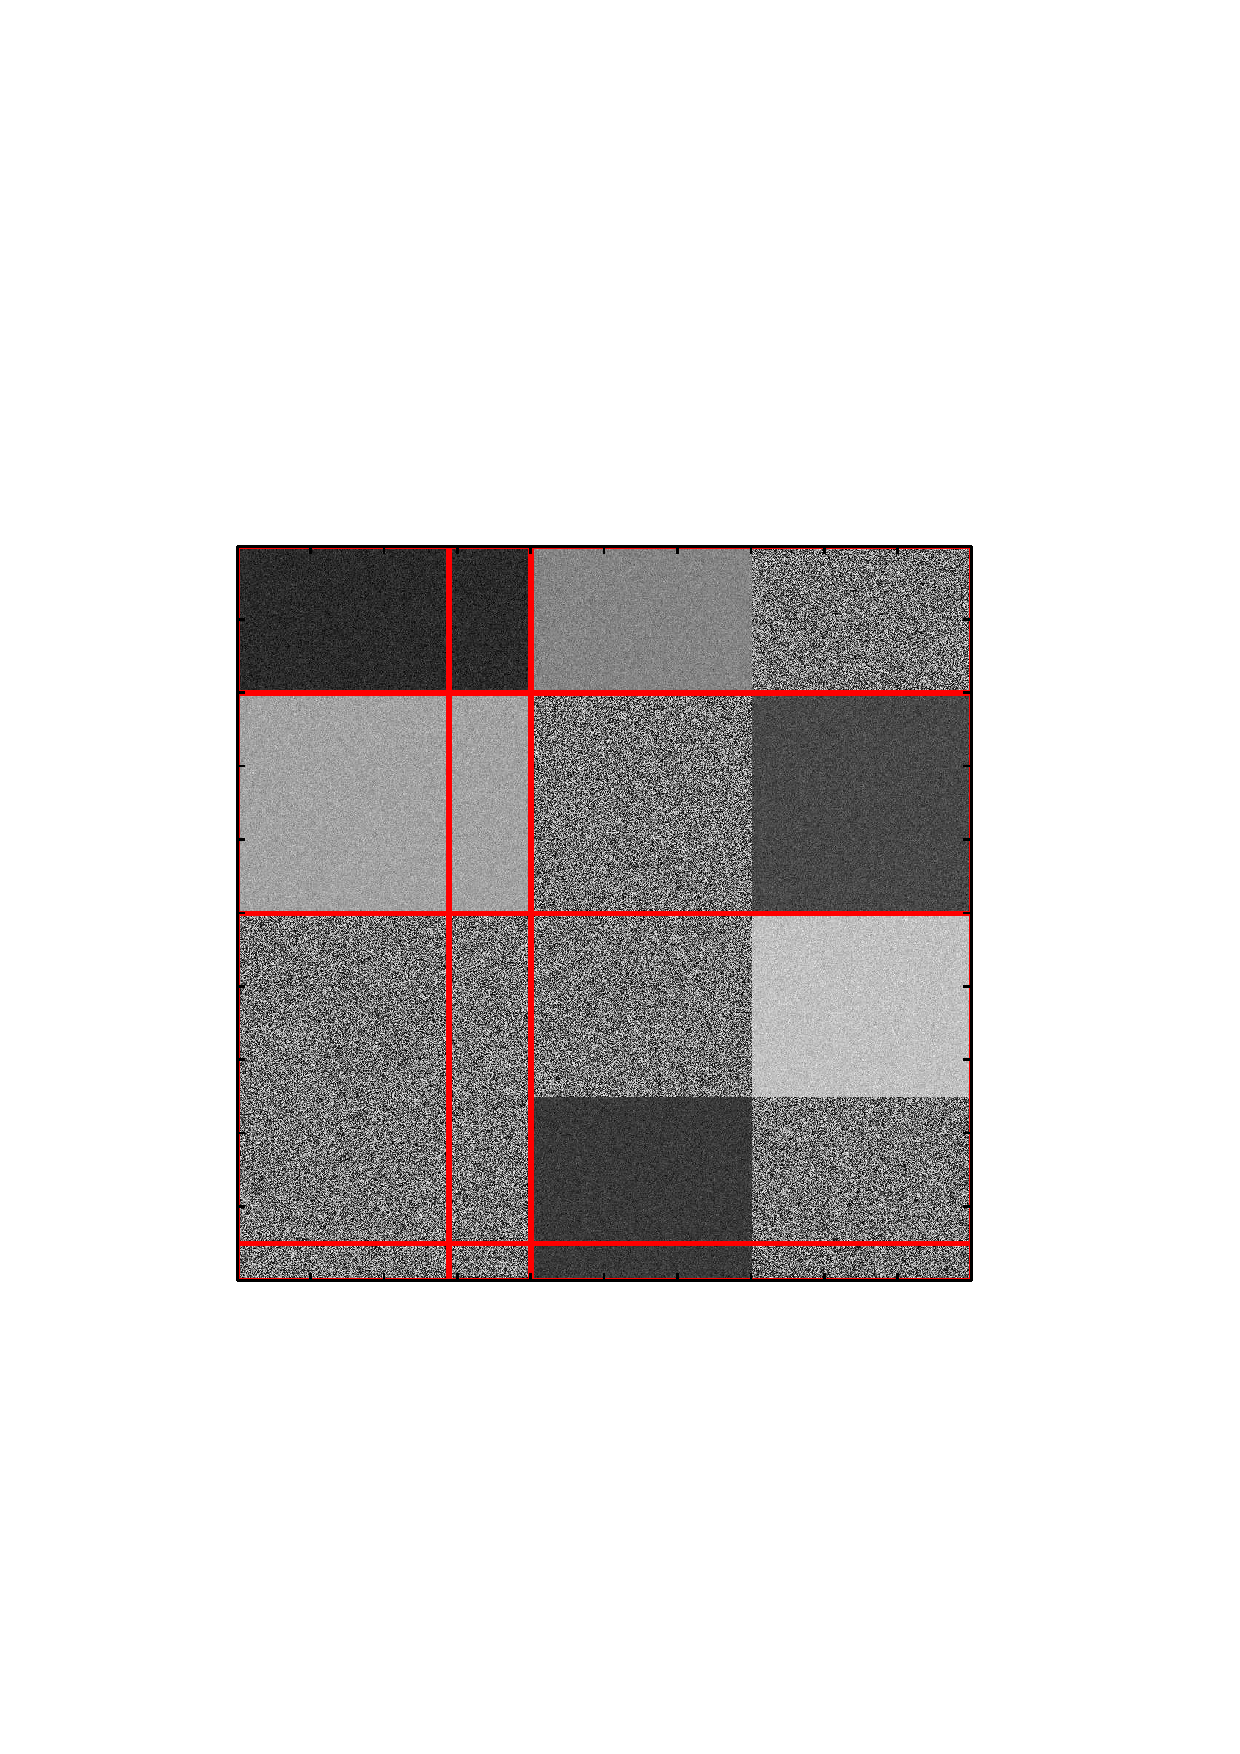
\includegraphics[width=45mm]{residue1}&
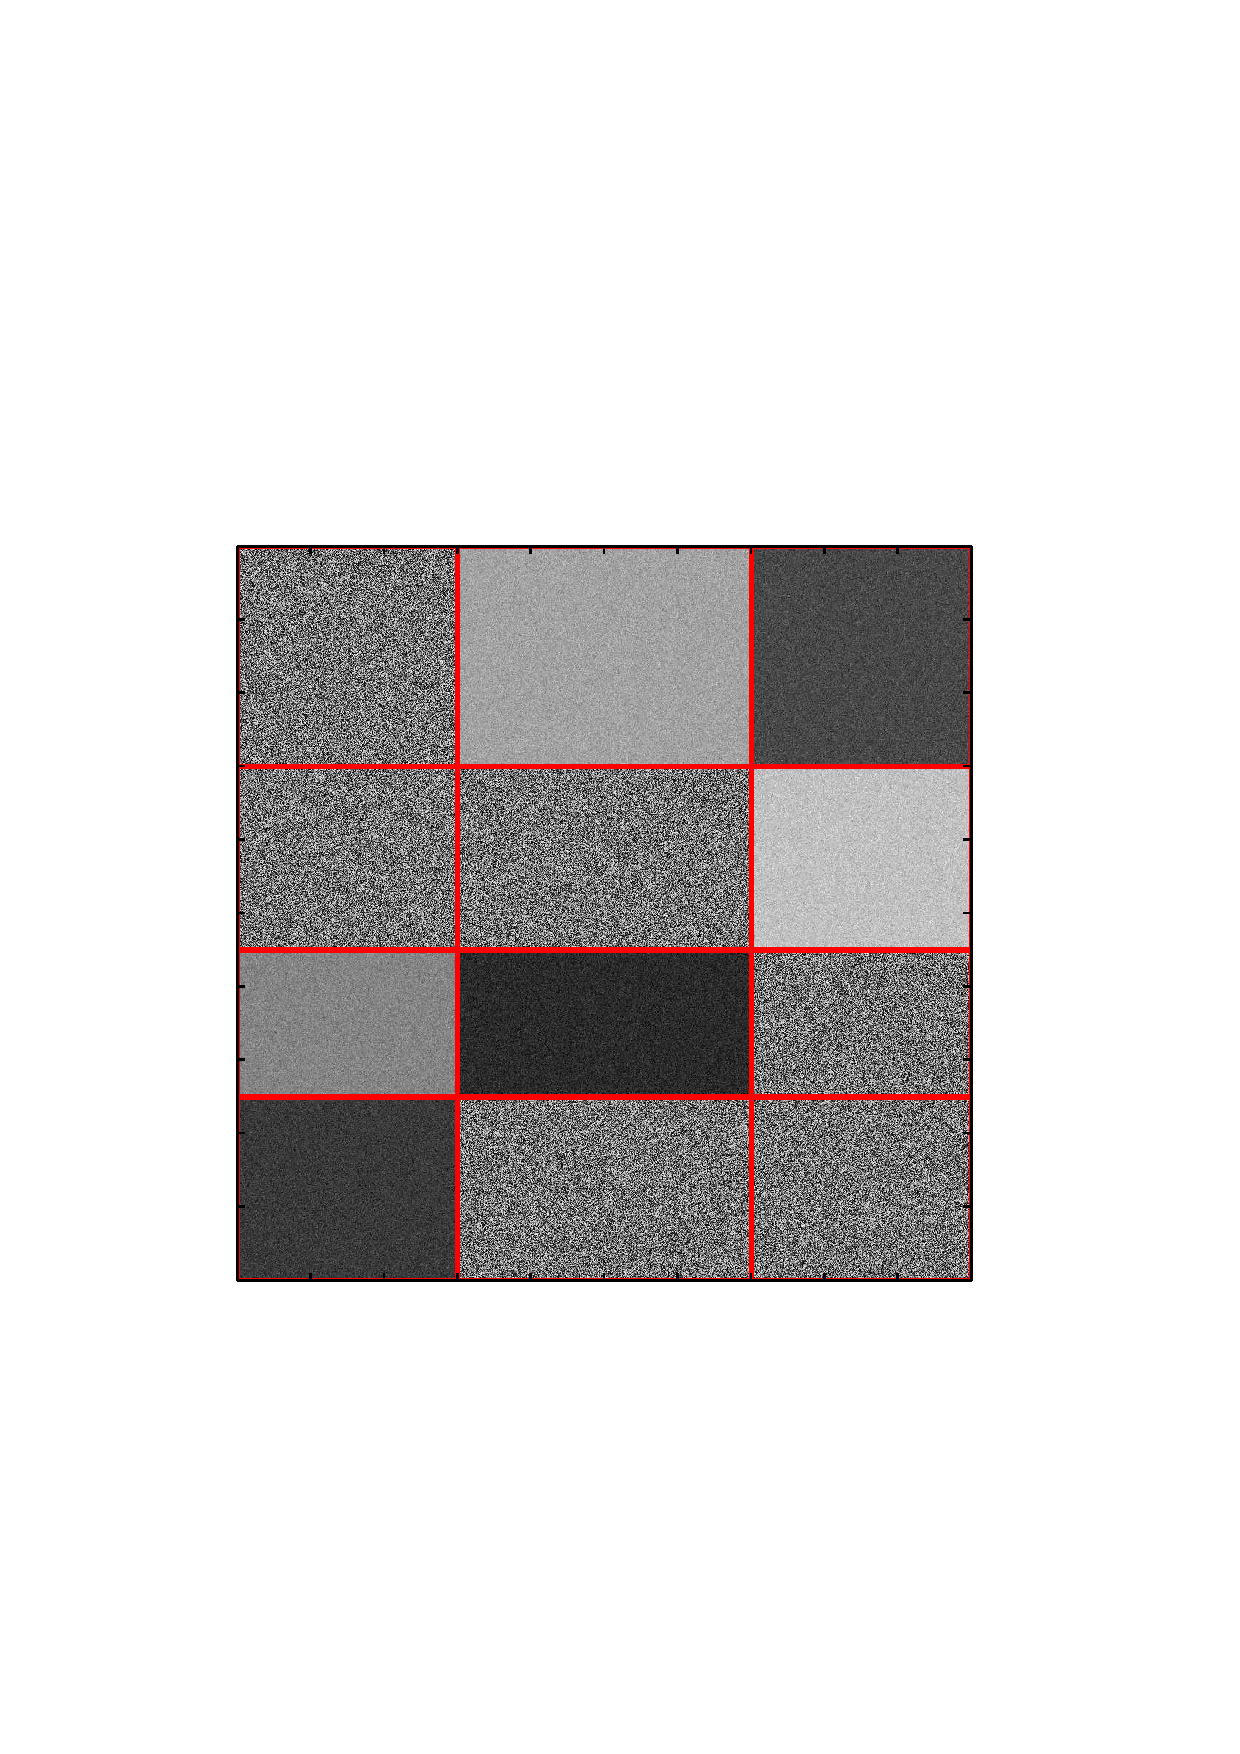
\includegraphics[width=45mm]{spectral1}&
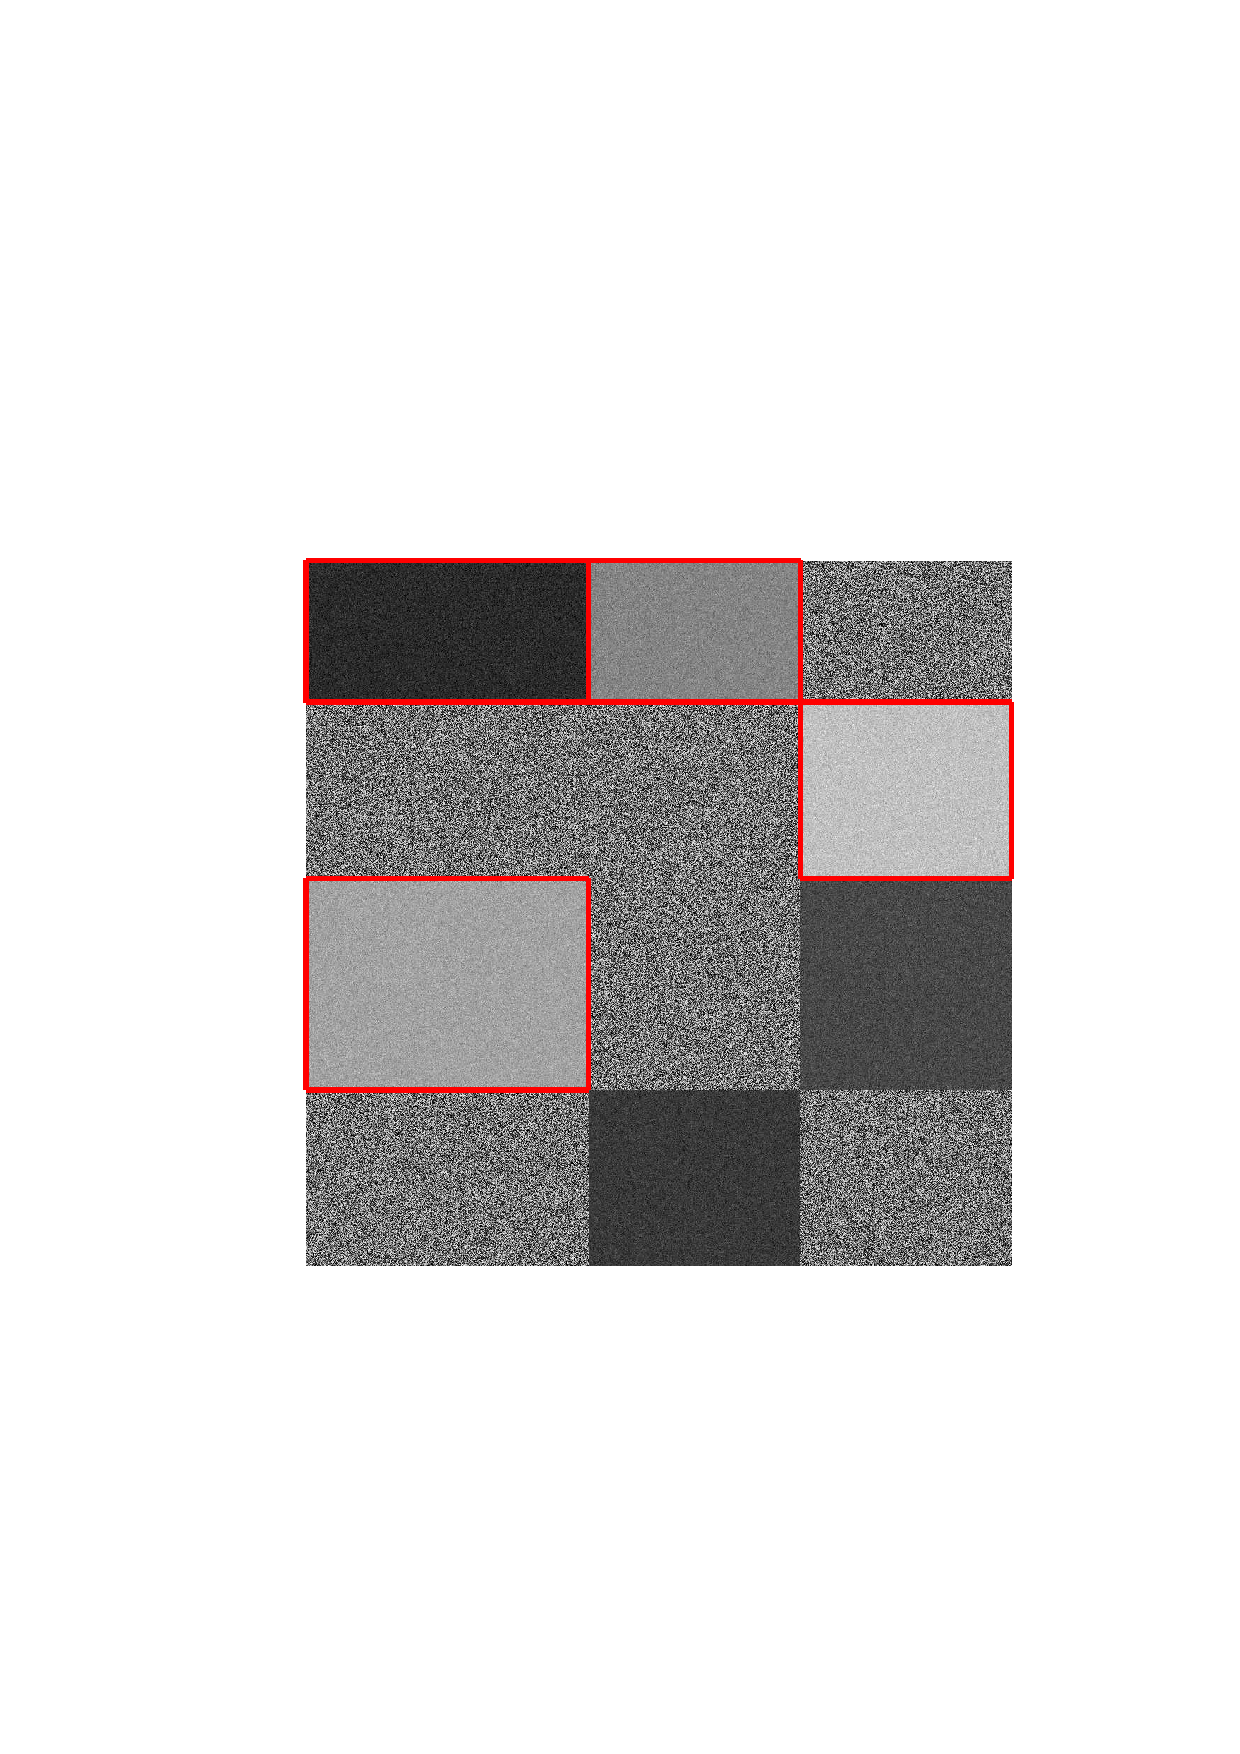
\includegraphics[width=45mm]{plaid1}\\
(d) MSSRCC &  (e)  Spectral &  (f) Plaid\\
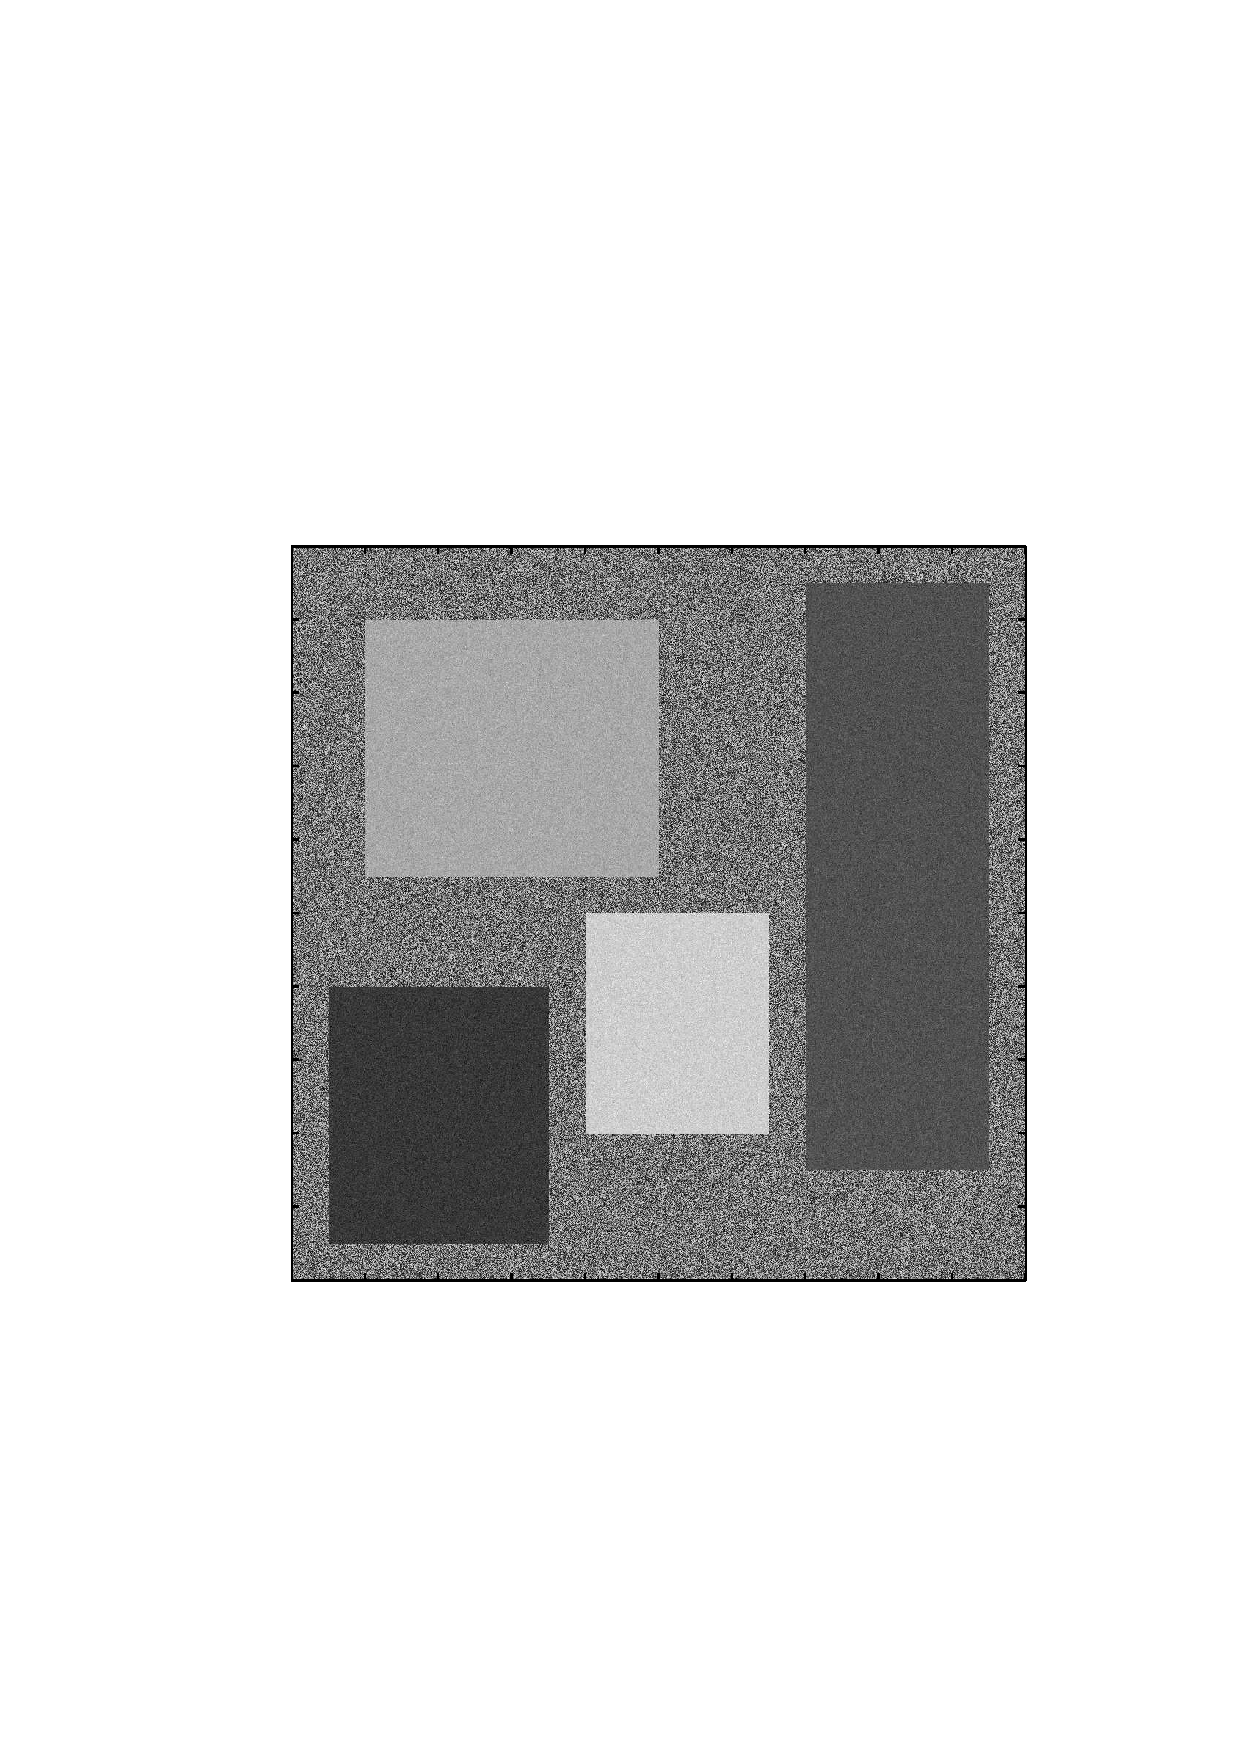
\includegraphics[width=45mm]{O2}&
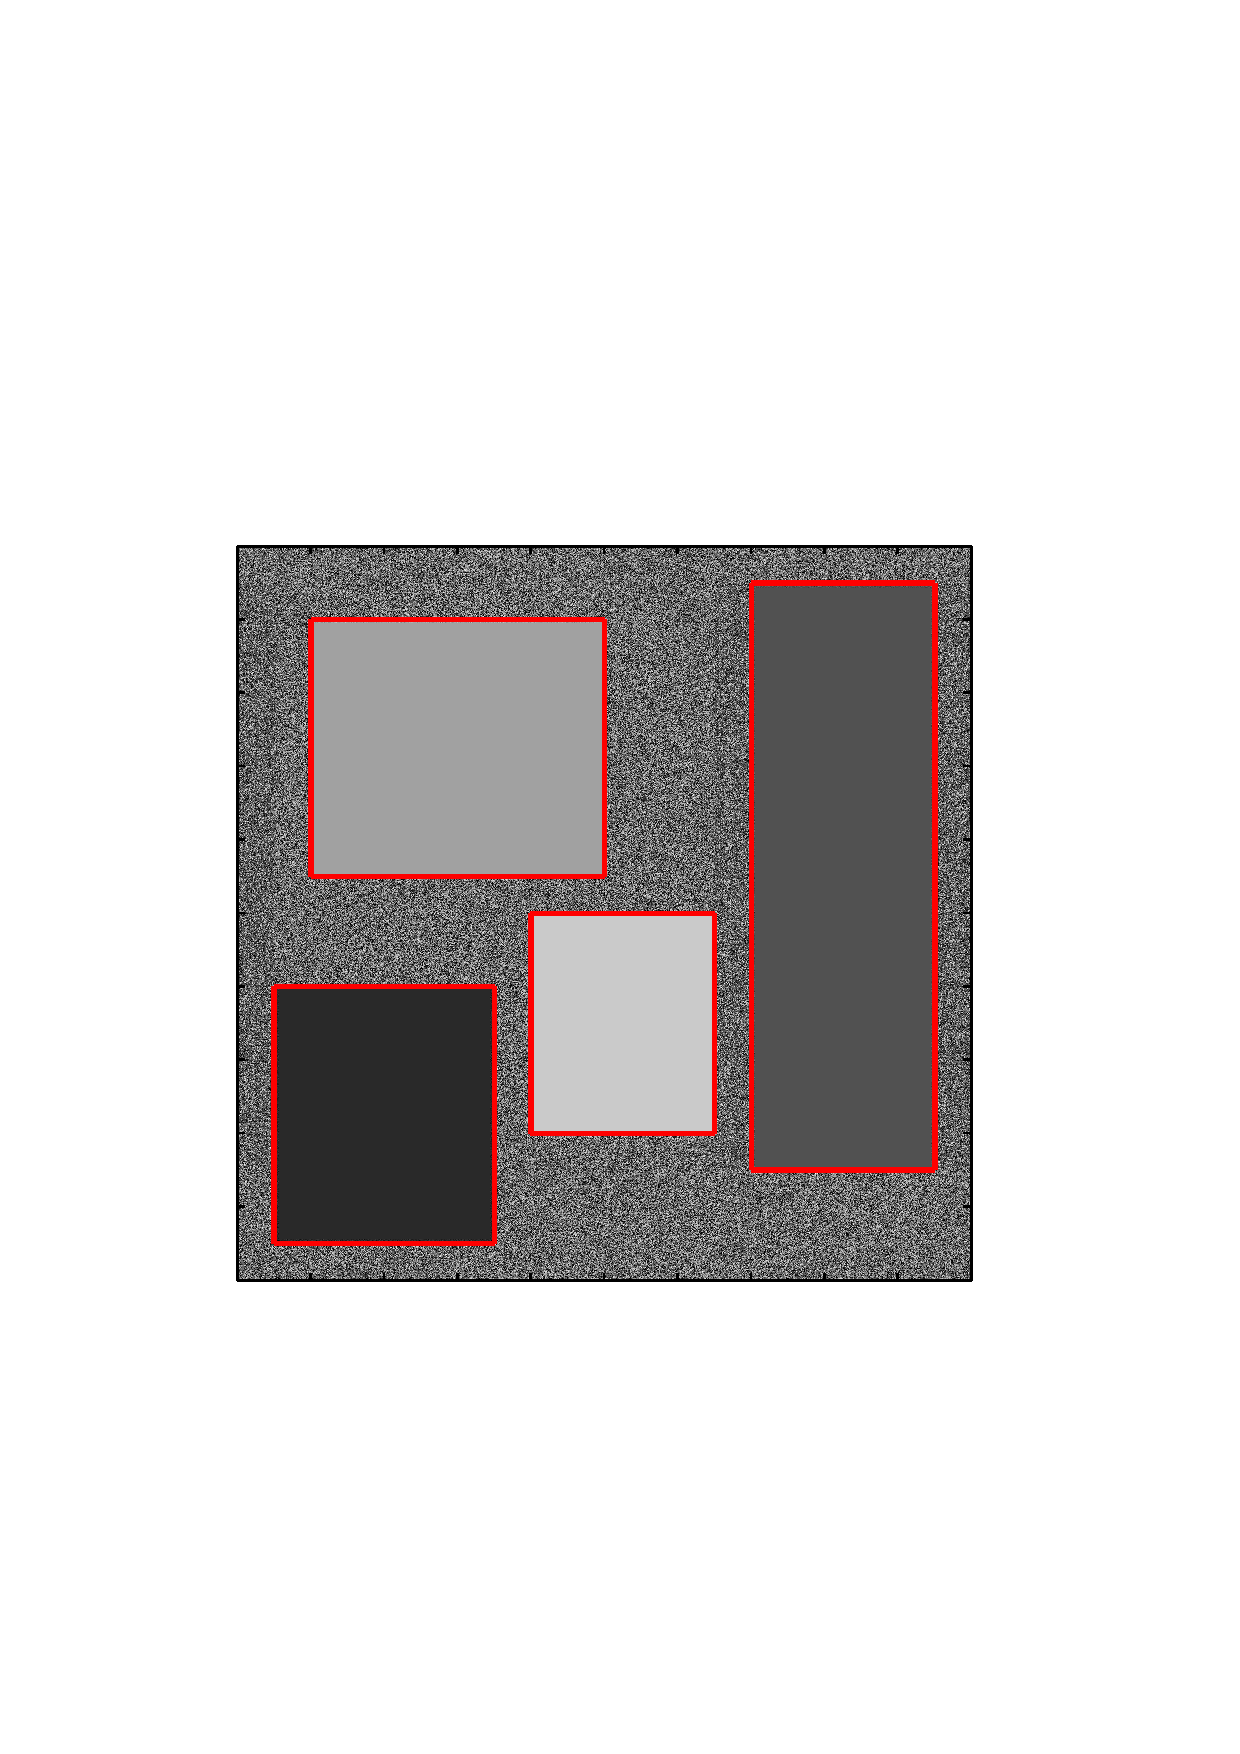
\includegraphics[width=45mm]{syn2R}&
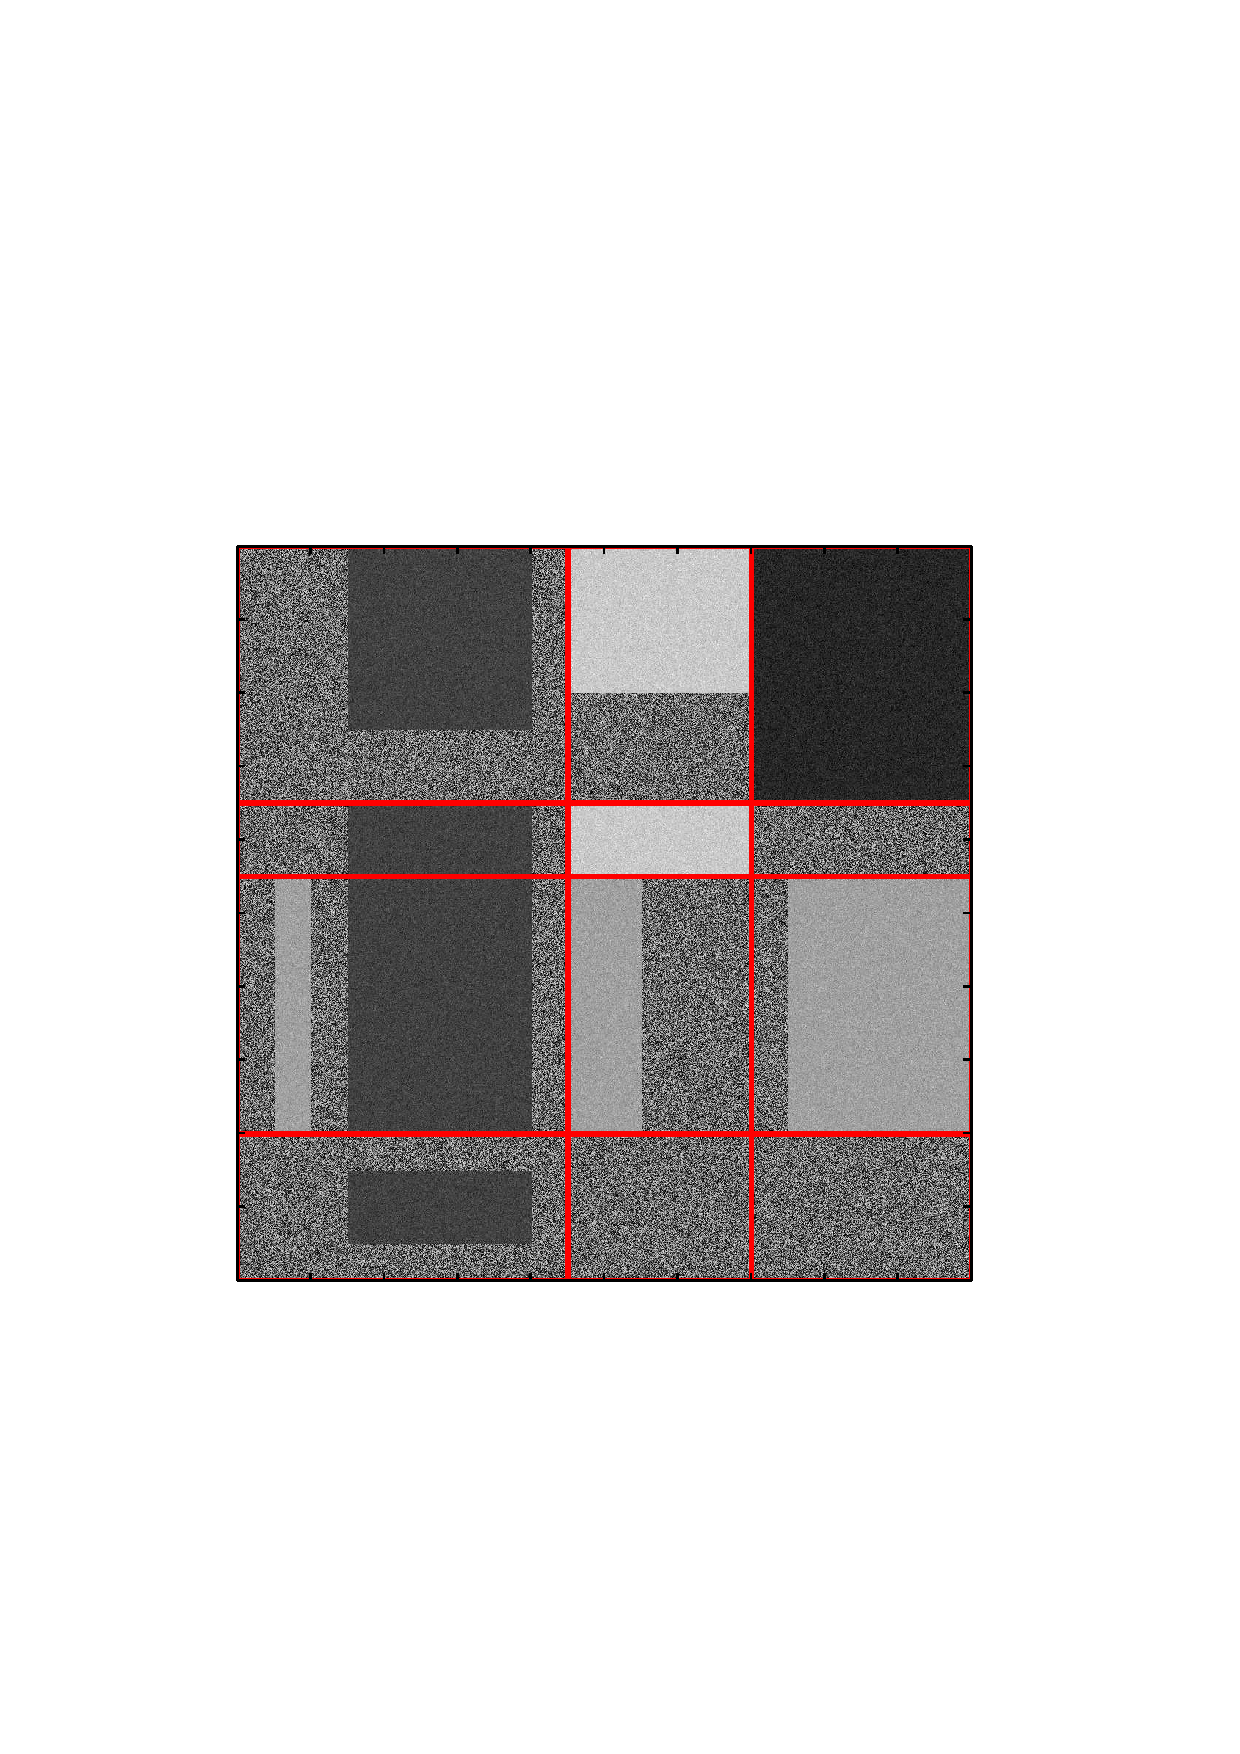
\includegraphics[width=45mm]{inf2}\\
(g) 随机分布矩阵  & (h) CoSync &  (i) ITCC\\
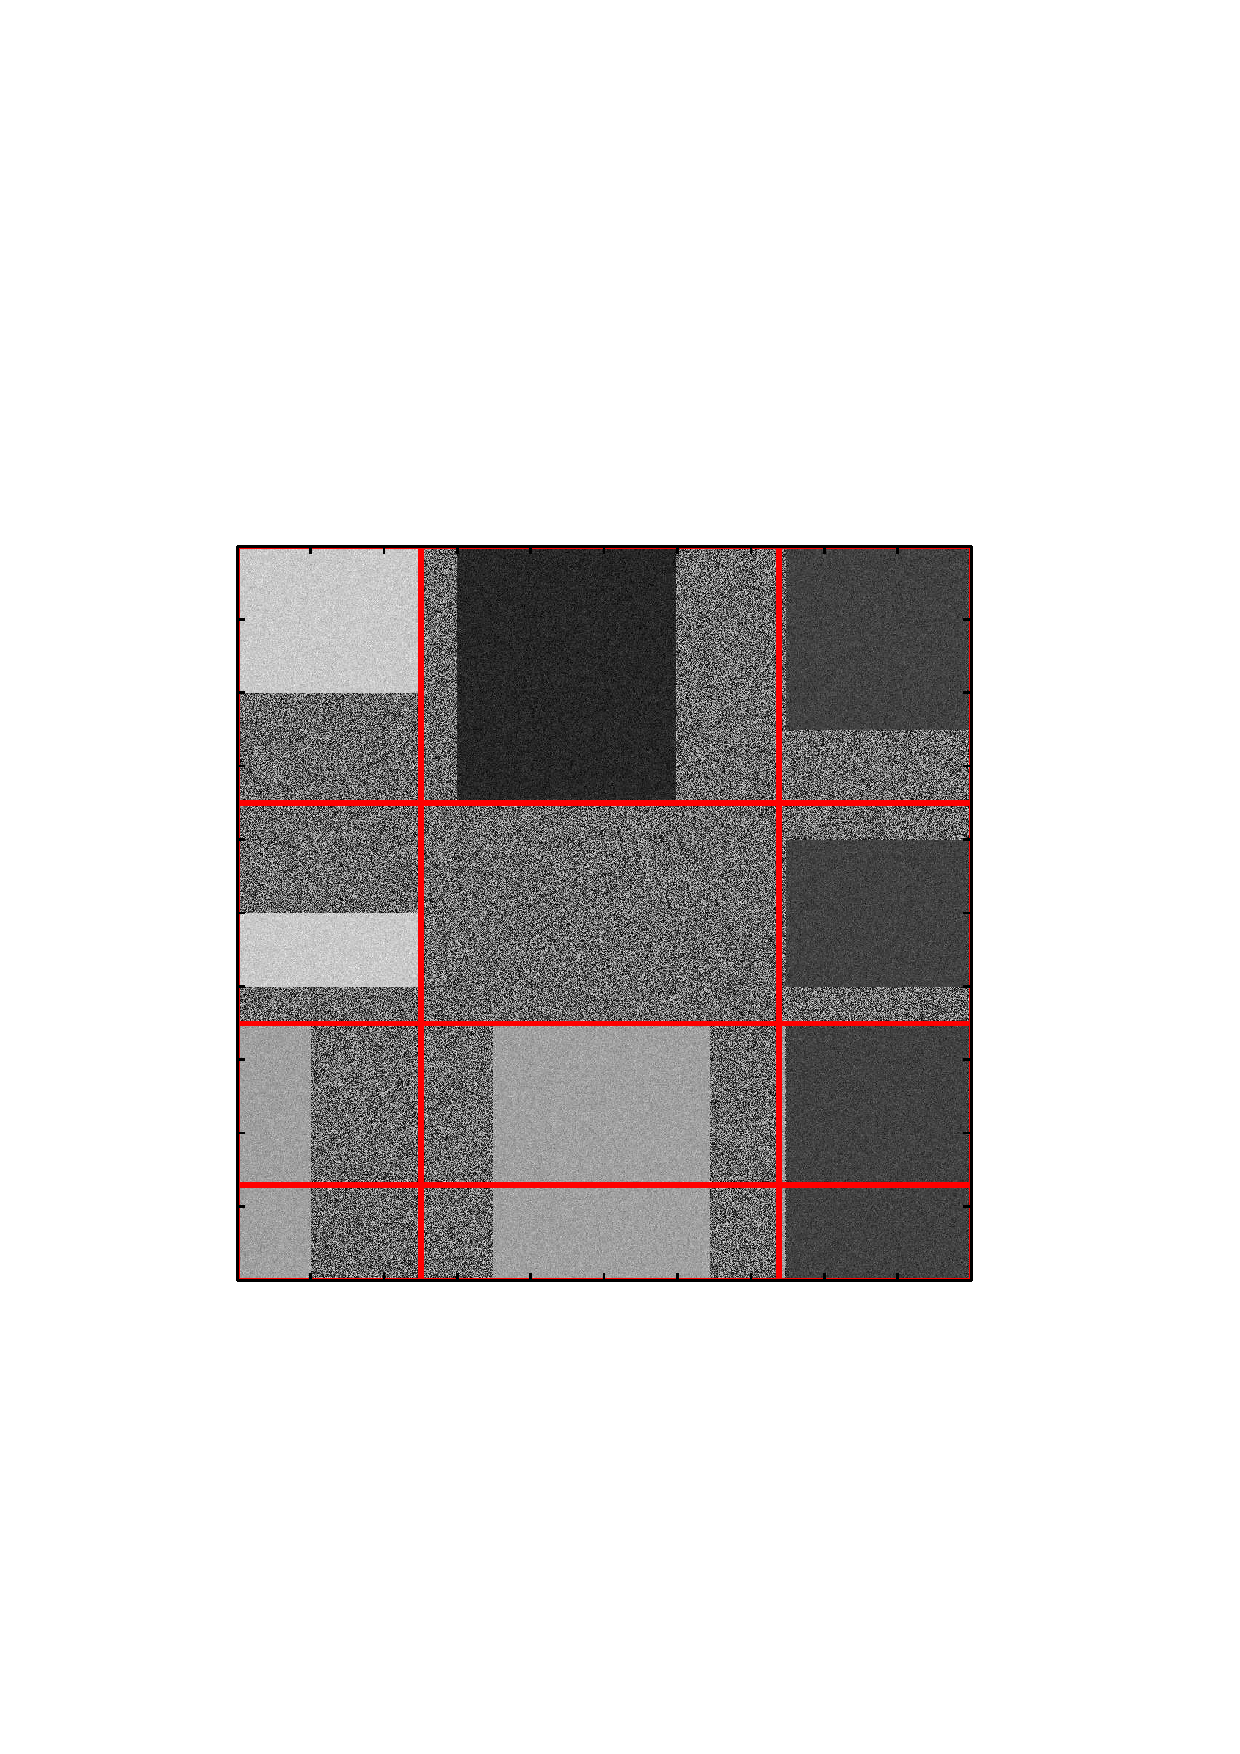
\includegraphics[width=45mm]{residue2}&
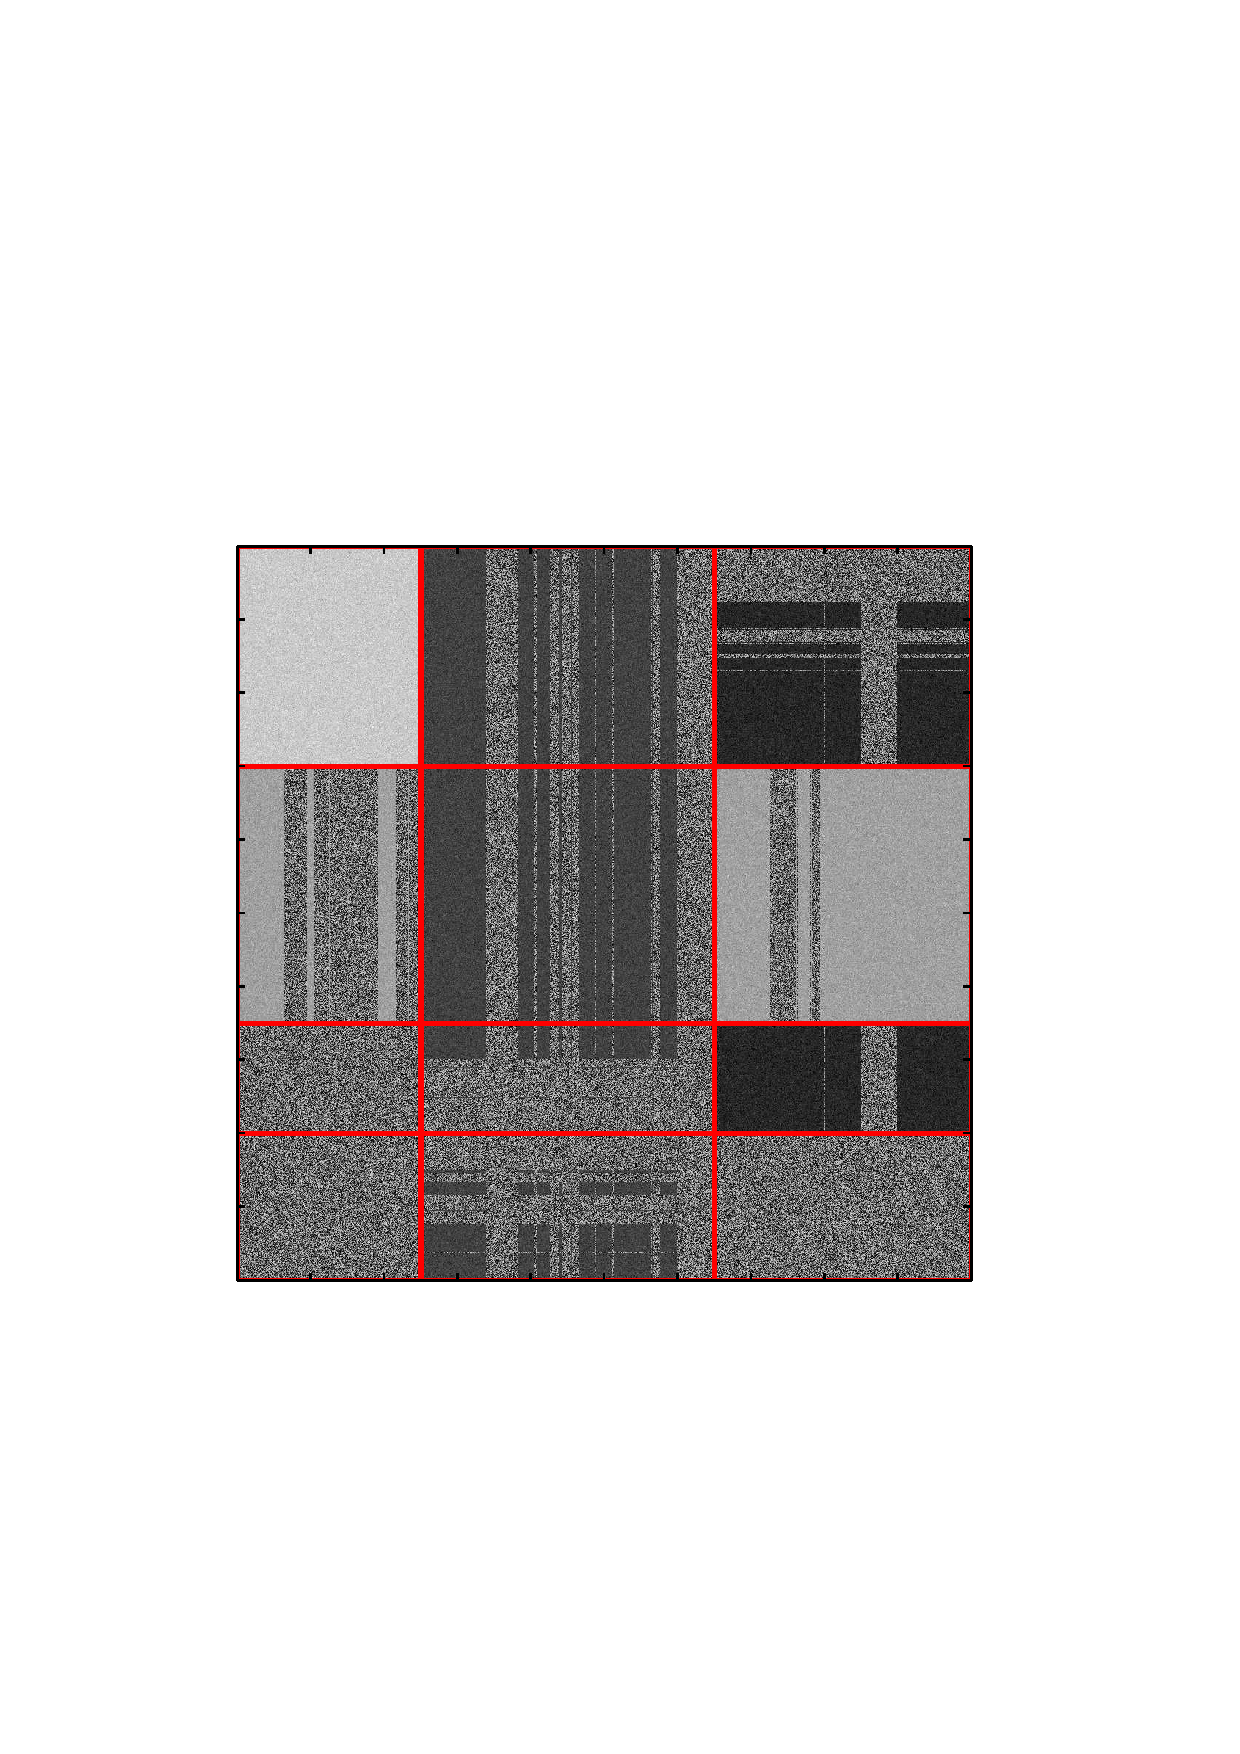
\includegraphics[width=45mm]{spectral2}&
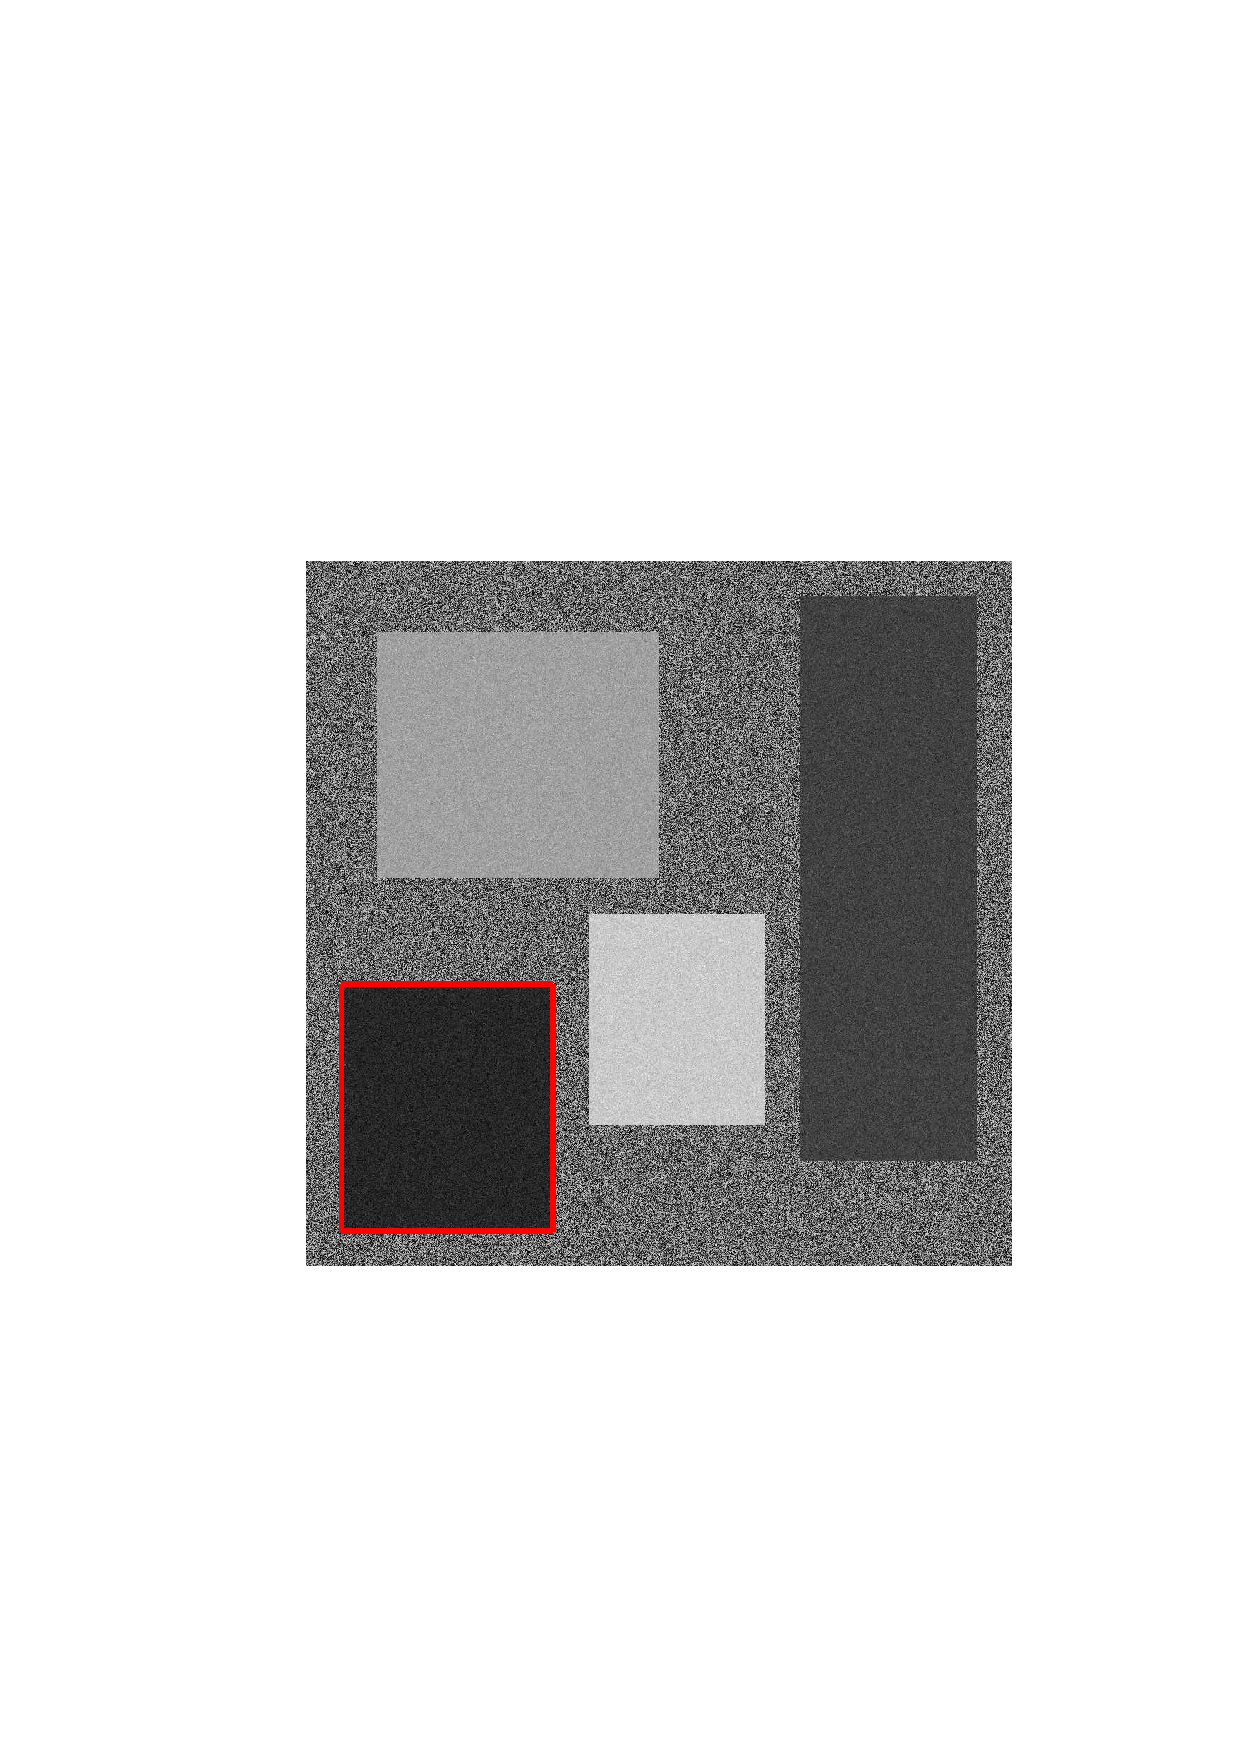
\includegraphics[width=45mm]{plaid2}\\
(j) MSSRCC &  (k)  Spectral &  (l) Plaid
\end{tabular}
\caption{五种算法在棋盘分布矩阵和随机分布矩阵上运行结果图。(a)为棋盘分布原矩阵。(b)-(f)为五种算法在棋盘分布矩阵上的聚类结果可视化。(g)为随机分布原矩阵。(h)-(l)是五种算法在随机分布矩阵上的聚类结果可视化。
图中红色方框为算法找出的聚类簇。}
\label{fig:yiqi_r}
\end{figure*}
% \pagenumbering{}

\vspace{3mm}
\textbf{棋盘分布下的算法比较}:
在本实验中,首先针对ITCC,MSSRCC和Spectral CLustering算法的特性,对棋盘式分布的矩阵进行测试。实验矩阵尺寸为$(1000\times1000)$,嵌入了6个从均值不同的高斯分布$N(\mu,\sigma)$中抽样的联合簇,其可视化图行列打散的的矩阵如图\ref{fig:yiqi}(a)-(b)所示。由于数据集的分布为棋盘分布,故行、列的划分数目很好确定,分别为$4$与$3$。

在5种算法完成测试后,各自得到输出的代表联合簇的行、列集合。我们对它们进行排序整理,重新规划为易于观察的矩阵,其可视化结果如图\ref{fig:yiqi_r}(b)-(f)所示。

图中红色方框为结果中识别出的聚类簇。可见只有\cosync和Plaid算法能够识别分散在矩阵中的聚类簇,其他三种对聚类簇的识别都是基于全局划分的。在图\ref{fig:yiqi_r}(b)中,可见\cosync算法分毫不差地挖掘出嵌入原始矩阵的6个联合簇,做到了识别度$100\%$;而在图\ref{fig:yiqi_r}(f)中,Plaid模型识别出了6个聚类簇中的4个,识别度为$66.6\%$。ITCC、MSSRCC与Spectral Clustering算法用划分的方式将原矩阵划分为$4\times3=12$块,图\ref{fig:yiqi_r}(c),(e)中ITCC和Spectral Clustering的12块子矩阵中成功地包括了嵌入的6块联合簇,而图\ref{fig:yiqi_r}(d)中的MSSRCC算法的划分没有成功地圈出联合簇。

总体来看,在这个实验集上,\cosync表现出了良好的特性,甚至胜出了专为棋盘式数据设计的ITCC,MSSRCC和Spectral Clustering算法。

\vspace{3mm}
\textbf{随机分布下的算法比较}:
在现实数据中,联合簇的嵌入不可能按照棋盘式方式规律分布,其分布是无规律而杂乱的。我们在本次实验中模拟了这种情况,将4个大小、尺寸不一致的联合簇随机嵌入$(1000\times1000)$的矩阵中,注意联合簇间不能互相遮挡重叠。其可视化图行列打散的的矩阵如图\ref{fig:yiqi}(c)-(d)所示。

同样地,5种算法在该数据集上运行完毕后,我们对各自输出的结果矩阵行列顺序整理重排,其可视化结果如图\ref{fig:yiqi_r}(h)-(l)所示。从结果中可以看出,\cosync算法依然准确地识别出了4个嵌入的联合簇,而Plaid算法仅识别出了1个联合簇。值得注意的是,在图\ref{fig:yiqi_r}(i)-(k)中的ITCC,MSSRCC和Spectral Clustering三种基于划分的方法此时已经失去效果。ITCC和Spectral Clustering仅划分出了一个联合簇。但由于受于方法本身的限制,它的划分不能将其余联合簇划分出来。MSSRCC则没有划分到正确的聚类簇。

在这次的比较中,\cosync发挥了其优势:能处理以任何分布方式的聚类簇,且发掘效果显著,胜出了其余几种代表性方法。

\subsection{人工数据集测试小结}
我们在本节的人工数据集测试中,首先用比较简单的$(100\times100)$数据集证明了\cosync算法的可行性,并作出数据集在同步过程中的变化图。接下来,在联合簇以棋盘方式和任意方式分布中大规模的$(1000\times1000)$数据集上,我们将\cosync算法和国际上比较有代表性的双边聚类算法ITCC,MSSRCC,Spectral Clustering和Plaid算法进行比较。两个的比较的结果中,\cosync都成功地识别出了矩阵中嵌入的所有联合簇,而其他算法都没有做到这一程度,这充分显现了\cosync算法在这一类数据集上的优势。总体来看,本次实验展示了\cosync算法的高效性和能抓住数据集本质结构的特性。

\section{基因表达数据上的算法实现及评估}
% \pagenumbering{arabic}
% \setcounter{page}{28}
\label{sec:gene}
在本小节中,我们将在基因数据集上对\cosync算法进行测试。首先我们将介绍选本次实验选用的基因数据集,之后给出\cosync运行的聚类簇可视化结果,最后根据生物信息学中对基因的评价方法来说明\cosync算法的运行结果。

\subsection{基因数据集选取}
DNA微阵列数据是一种观测基因在特定样本上表达程度的数据\footnote{\url{https://en.wikipedia.org/wiki/DNA_microarray}},可以用一个矩阵来表示,其中行代表基因,列代表特定样本,如不同个体,不同组织,或者不同环境下观测到的数据。

本文第一章提过,双边聚类这一领域就是在基因数据集上发展起来的,后面只有少部分方法能扩展到购物篮数据集以及文本-词汇数据集上。导致这一现象的原因是现实情况中,只有基因数据集密集无缺失值,这是距离度量的必要条件。

在本章第\ref{subsec:principle}节中的数据集选取原则中提到,\cosync可以处理的数据集必须是数值型无缺失值的,基因数据集满足这一条件。然而基因数据集的尺寸规模几乎都为$1000\times10$量级,即数千规模的基因在数十个样本上的表达程度,使得矩阵的行列比例严重失调。前文说过,数据集比例失调可能会带来算法正确率降低。面对这一困扰,我们只能在实验中尽量以调参数的方式来进行应对。

本次实验中,我们选取了四个通用的基因表达数据集\footnote{基因数据集矩阵及对应的基因名称来源:\url{http://datam.i2r.a-star.edu.sg/datasets/krbd/index.html}},皆被国际众多知名双边聚类算法所使用,其信息总结如表\ref{tab:dataset}。
\vspace{3mm}
\tabcolsep=5pt
\begin{table}[!htb]\renewcommand{\arraystretch}{1.3}
\center \caption{四个基因数据集的统计信息表}
\small
\begin{tabular}{c|c|c|c|c}
\hlinew{1pt}
\textbf{数据集}& \#\textbf{基因数目}& \#\textbf{样本数目} & \textbf{样本类别名称}&  \textbf{样本分布}\\
\hlinew{1pt}
Colon  &  1096 & 62 &Normal/Tumor& 20/42  \\ \hline
Leukemia   & 3571 & 72 &ALL/AML & 47/25    \\ \hline
Lung    & 2401 & 181 &ADCA/MPM& 150/31 \\ \hline
MLL & 2474 & 72  & ALL/AML/MLL&24/28/20 \\ \hlinew{1pt}
\end{tabular}
\label{tab:dataset}
\end{table}

可见数据集的行列比例很不均衡。其样本类别只有两个或者三个,其中ALL、AML、ADCA、MPM和MLL均为疾病名称的缩写,而基因没有直接的类别标签。
%其结果评价将用\ref{subsec:analysis}中所述的基因集丰富度分析来进行。

\subsection{\cosync在基因数据集上的联合簇挖掘}
真实数据集与人工数据集的差别在于真实数据集的联合簇数目更多、大小更不规律、分布更不均衡,取不同的$\epsilon$邻域邻居将得到不同层次下的联合簇。我们结合专家知识来制定合适的$\epsilon$取值范围,在取值范围内用\cosync对上述数据集进行多次测试后,得到一些特定值的大尺寸联合簇。

我们将\cosync,ITCC,MSSRCC,Spectral Clustering和Plaid算法在四个数据集上进行了实验。如前文所述,基因空间的评价无法直接对比,其将用\ref{subsec:analysis}中所述的基因集丰富度分析来来进行。故我们仅将对他们找出的联合簇中的样本空间进行评价对比,用\ref{subsec:evaluation}节中叙述的准确率和召回率作为评价指标。表\ref{tab:compare}展示了四种算法在四个数据集上找到的所有联合簇在样本空间中的评价。

\vspace{2mm}
\tabcolsep=3pt
\begin{table}[!htb]\renewcommand{\arraystretch}{1.2}
\center \caption{五种算法在四个数据集上找出聚类簇的样本空间评价}
\small
\begin{tabular}{c|ccc|ccc|cc|cc|cc}
\hlinew{1pt}
\multirow{2}{*}{\textbf{}} & \multicolumn{3}{c|}{\textbf{ CoSync}}&\multicolumn{3}{c|}{\textbf{Plaid}}& \multicolumn{2}{c|}{\textbf{ ITCC}} &\multicolumn{2}{c|}{\textbf{ MSSRCC}} & \multicolumn{2}{c}{\textbf{ Spectral}}  \\
\cline{2-13}
  & \#C &Pre. & Rec. & \#C &Pre. & Rec. & \#C & Avg. &\#C & Avg. &\#C & Avg. \\[0.4ex] \hlinew{1pt}
Colon & 11& 0.95 & 0.66& 4&0.71&0.66& 2& 0.82& 2& 0.86 &2 & 0.73\\
Leukemia & 28& 0.96 & 0.71 &2&0.81&0.43& 2& 0.95&2 & 0.93&2 & 0.74\\
Lung& 23& 1.00& 0.96 &3&1.00&0.50& 2& 0.85& 2& 0.99& 2& 1.00 \\
MLL& 23& 0.99 & 0.67 &4&0.88&0.88&3 &0.83 &3 &0.93 &3 &0.64 \\ \hlinew{1pt}
\end{tabular}
\label{tab:compare}
\end{table}

可以看到ITCC,MSSRCC和Spectral Clustering算法的由于基于划分,故其样本空间划分数目已经提前被指定好,均为数据中样本类别的真实数目。在自动找寻联合簇的算法\cosync和Plaid当中,Plaid找出的簇仅为$2\sim4$个,而\cosync算法在Colon数据集中找出11个联合簇,而其他三个数据集上,都发掘出了$20$个以上的联合簇。

关于样本的评价标准,\cosync在四个数据集上准确率都达到了令人满意的$95\%$以上,而召回率达到了$66\%$以上。这说明了\cosync算法找出的联合簇都能代表真实数据中的数据结构。而召回率在这重要性不是很高,因为这仅代表着算法找出的样本没有覆盖整个样本维空间。从准确率上来看,其他算法的性能都没有超过\cosync,而从召回率的角度看,基于划分的方法明显超出\cosync算法,这是合理的结果。

其次,我们还能从图中看出,数据集Lung在五个算法下都表现出了优良的性能,而Colon数据集在5个算法下的性能都不如其他数据集。这说明数据集本身的结构会影响所有的算法效能。

为了观察\cosync找出的聚类簇的具体形态,我们为上述结果中\cosync的前十大尺寸的聚类簇进行更细的观察。表\ref{tab:real}列举了四个数据集中尺寸最大的10个联合簇的信息,包括该联合簇的行、列数目,以及关于样本维度上的精确率和召回率。




从表中的结果中我们可以看出来,\cosync的找寻质量还是较高的。大多数聚类簇的准确率都是$1.00$,在Lung数据集上甚至所有的聚类簇在样本维空间上的聚类准确率都为$1.00$。这一结果更肯定了我们上述的判断:\cosync算法找出的聚类簇的准确率很高。

ITCC,MSSRCC和Spectral Clustering算法这样基于划分的方法在没有标签的情况下, 决定划分簇数目是非常困难的,错误的参数指定将会带来完全偏离真实情况的结果。接下来,我们将对五种算法找出的联合簇对基因维度进行评价。

\subsection{基因集丰富度分析}
\label{subsec:analysis}
我们实验数据的基因表达数据来源于对数以千的基因在特定样本下进行表达的探测。这其中样本的分类是明确的,但是基因却没有确定的类标签。为了衡量数据挖掘、人工智能算法对基因分类、聚类的结果,一种专门的衡量指标被提了出来,即基因集丰富度分析。

基因丰富度分析\footnote{\url{https://en.wikipedia.org/wiki/Gene_set_enrichment}},也称为功能性丰富度分析,是一种为基因和蛋白质的归类显著性进行评判的一种分析方法。基因没有类标签,但大量的实验表明在一些特定的试验下,观测基因经历一些生物过程最终表达为蛋白质的情况,一部分基因会表达得更明显,而另外的基因则被抑制或不表达。搜集这些历史记录,大量的特定的基因集合被记录下来,它们被记录在基因本体库\footnote{\url{https://en.wikipedia.org/wiki/Gene_ontology}}中。基因本体库中的特定基因集合可以分为以下三个邻域类别:
\begin{itemize}
\item \textbf{~~细胞组件(cellular component)}:细胞的每个部分和细胞外环境。
\item \textbf{~~分子功能(molecular function)}:基因产物在分子级别的主要活动,比如结合以及催化。
\item \textbf{~~生物过程(biological process)}:细胞内发生的,可以定义开始和结束的事件或行动。
\end{itemize}

有了基因本体库,我们用算法对基因进行聚类的结果便有了比对的参照物。针对我们算法找出的基因数据集与基因本体中不同情况下的基因集合,用假设假设检验\footnote{\url{https://en.wikipedia.org/wiki/Statistical_hypothesis_testing}}的方式,便能得知我们找出的基因集合是否合理:是否完全属于某一个基因本体中的基因集合?是否太过随机,没有任何代表性?用这种方式,我们便能评价\cosync找出的聚类簇中基因空间中的结果好坏。

\tabcolsep=4pt
\begin{table*}[!h]\renewcommand{\arraystretch}{1.2}
\center \caption{各个数据集上前十大联合簇信息。其中 $P$ 和 $R$ 分别代表每个联合簇在样本空间中的精确率和召回率。 $No.G.$ 和 $No.S.$分别是联合簇包含的基因和样本的数目。 $N$ 和 $T$ 分别代表Colon数据集中的Normal和Tumor。 $A$ 和 $M$ 分别代表Lung数据集中的ADCA和MPM。 $AL$, $AM$ 和 $ML$ 分别代表Leukemia和MLL数据集中的ALL,AML和MLL。}
\small
\begin{tabular}{ccccccccccccc}
\hlinew{1pt}
&~~&\multicolumn{5}{c}{\textbf{Colon}} & &\multicolumn{5}{c}{\textbf{Leukemia}} \\ \cline{3-7} \cline{9-13}
 \textbf{cID} &~~& \textbf{Size}   &\textbf{No.G. }& \textbf{No.S. } & \textbf{P} &\textbf{R}&~~& \textbf{Size}   &\textbf{No.G.} & \textbf{No.S.}  & \textbf{P} &\textbf{R}\\
\hlinew{1pt}
1   &~~& 1480  &296   & 5(N)   &1.00  & 0.23 &~~&3216 & 268 & 12(7AL/5AM) &0.58  &  0.15  \\
2   &~~& 966   &138   &7(5N/2T)&0.71  & 0.23 &~~&2570 &514  & 5(4AM/1AL)  &0.80  &0.16    \\
3   &~~& 666   &111   &6(T)    &1.00  &0.15  &~~&2320 &464  & 5(AL)        &1.00  &0.11   \\
4   &~~& 510   &85    &6(5N/1T)&0.83  &0.23  &~~&1480 &296  & 5(AL)        &1.00  &0.11   \\
5   &~~& 420   &84    &5(N)    &1.00  &0.13  &~~&1215 &243  & 5(AM)        &1.00  &0.20   \\
6   &~~& 290   &58    &5(T)    &1.00  &0.13  &~~&625  &125  & 5(AL)        & 1.00 &  0.11 \\
7   &~~& 205   &41    &5(T)    &1.00  &0.13  &~~&320  &64   &5(AL)         &1.00  &0.11   \\
8   &~~& 125   &25    &5(T)    &1.00  &0.13  &~~&294  &49   &6(AM)         & 1.00 &0.24   \\
9   &~~& 65    &13    &5(T)    &1.00  &0.13  &~~&264  &22   &12(AL)        &1.00  &0.26   \\
10  &~~& 49    &7     &7(T)    &1.00  &0.13  &~~&242  &22   &11(AL)        & 1.00 &  0.23 \\
\hlinew{1pt}


&~~&\multicolumn{5}{c}{\textbf{Lung}} & &\multicolumn{5}{c}{\textbf{MLL}}\\ \cline{3-7} \cline{9-13}
 \textbf{cID} &~~&  \textbf{Size}   &\textbf{No.G.} & \textbf{No.S.}   & \textbf{P}&\textbf{R}&~~&  \textbf{Size}   &\textbf{No.G.} & \textbf{No.S.}   & \textbf{P }&\textbf{R}\\
 \hlinew{1pt}
1  &~~& 5614   & 401  & 14(A)   & 1.00  & 0.09 &~~&4228   & 302  & 14(AM)   & 1.00      & 0.50  \\
2  &~~& 4394   & 338  & 13(M)   & 1.00  & 0.42 &~~&3765   & 251  & 15(AL)   & 1.00      & 0.63  \\
3  &~~& 3960   & 264  & 15(A)   & 1.00  & 0.10 &~~&2954   & 211  & 14(AL)   & 1.00      & 0.58  \\
4  &~~& 3806   & 346  & 11(M)   & 1.00  & 0.36 &~~&2071   & 109  & 19(AM)   & 1.00      & 0.68   \\
5  &~~& 2344   & 293  & 8(A)    & 1.00  & 0.05 &~~&1584   & 99   & 16(AM)   & 1.00      & 0.57  \\
6  &~~& 2210   & 221  & 10(M)   & 1.00  & 0.32 &~~&918    & 102  & 9(AL)   & 1.00      & 0.38   \\
7  &~~& 1770   & 177  & 10(M)   & 1.00  & 0.32 &~~&890    & 89   & 10(AL)   & 1.00      & 0.42   \\
8  &~~& 1035   & 115  & 9(M)    & 1.00  & 0.29 &~~&715    & 143  & 5(3ML/2AL) & 0.60  & 0.15   \\
9  &~~& 950    & 190  & 5(A)    & 1.00  & 0.03 &~~&533    & 41   & 13(AM)   & 1.00      & 0.46   \\
10 &~~& 420    & 30   & 14(M)   & 1.00  & 0.45 &~~&510    & 34   & 15(AM)   & 1.00      & 0.54   \\

\hlinew{1pt}

\end{tabular}
\label{tab:real}
\end{table*}

统计假设检验用p-value\footnote{\url{https://en.wikipedia.org/wiki/P-value}}来作为显著与否的评价指标。其概念定义如下:

\textbf{显著性因子p-value}:一种在原假设为真的前提下出现观察样本以及更极端情况的概率。设某假设为$H_0$,则p-value在$H_0$为真的条件下,因样本偏差太大而拒绝$H_0$的概率,即:
\begin{equation*}
p-value = P(\text{拒绝接受}H_0\big{|}H_0\text{为真})
\end{equation*}

p-value值越小,则说明拒绝$H_0$的概率越小,也就是假设$H_0$越可信。当p-value取$0$时候,假设$H_0$与观测相比毫无差别。而当p-value值打过一定程度时候,结果就不可信了。对此人们通常设置一个阈值$\alpha$,当$p-value\ge\alpha$时,便拒绝假设$H_0$。

\vspace{2mm}
在基因库丰富度分析中,令真实的一个基因集合为$\mathcal{G}$,而预测出来的基因集合为$\hat{\mathcal{G}}$,对应假设$H_0$的命题为:
\begin{equation*}
H_0 = \{\hat{\mathcal{G}}\subseteq{}\mathcal{G}\}
\end{equation*}

即p-value在基因库丰富度分析中,可以作为任意给定的基因集合的显著性的指标。由此我们可以预先设置一个拒绝阈值:$\alpha$,之后对每一个聚类簇的基因与基因本体中每一个基因集合对比,算出一个对应的p-value值,若其大于$\alpha$,则不考虑基因本体中这个基因库。最后我们对基因本体库中的满足$p-value\leq\alpha$的基因集合列举出来。我们的算法找出的基因簇很可能就是这些基因集的子集。

值得说明的是,给定我们的基因集合,对基因本体库里任意的基因集合都能算出一个p-value,虽然这些p-value本身值越小越好,但它们互相之间是不可比较的。例如我们不能因为我们的基因集对与艾滋病蛋白相关的基因本体集的p-value比其于白血病蛋白相关的基因本体集的p-value值小,就说明我们的基因集更倾向于与艾滋病的蛋白表达相关。也正是这个原因,有三个浅显的结论:
\begin{itemize}
\item ~~不同算法间找出聚类簇中基因集合的p-value值之间不能相互比较。
\item ~~同一算法中,不同聚类簇基因集的p-value值不能相互比较。
\item ~~同一算法中,同一聚类簇中的基因集对基因本体中不同基因集的p-value值之间不能相互比较。
\end{itemize}

由于\cosync与其他算法找出聚类簇的基因集显著结果无法比较,故本文中我们仅对我们的\cosync算法进行基因集丰富度分析。表

\tabcolsep=1pt
\begin{table*}[!htb]\renewcommand{\arraystretch}{0.9}
\center \caption{\cosync算法找出的联合簇在基因空间上丰富度分析结果表。这里 BP 代表 “Biological Process”,CC 代表 “Cellular Component”。 \#Annotations 代表 p-value $<$0.05的所有基因本体库中的基因集数目。}
\scriptsize
\begin{tabular}{c|c|cclccc}
\hlinew{0.85pt}\textbf{Data Sets} &\textbf{ CluID} & \#\textbf{Genes} & \#\textbf{Annotations}&\textbf{Top Enriched Annotations} &\textbf{Count} & \textbf{Percentage (\%) } & \textbf{P-Value}  \\[0.4ex] \hlinew{0.85pt}

%Colon
\multirow{12}{*}{Colon} &\multirow{4}{*}{C1}& \multirow{4}{*}{296} &\multirow{4}{*}{214}& CC:cytosol                &34  & 23.61\%   & 5.84E-07\\
&&&&CC:plasma membrane part    &42  & 29.17\%    &3.01E-05\\
&&&&BP:negative regulation of molecular function          &13  &9.03\%     &7.69E-05\\
&&&& BP:striated muscle tissue development          &8  &5.56\%     &1.34E-04\\
\cline{2-8}
 &\multirow{4}{*}{C2}& \multirow{4}{*}{138} &\multirow{4}{*}{157}& CC:plasma membrane part & 22 &37.29\%& 4.81E-05\\
&&&& CC:plasma membrane& 28 &47.46\%&3.87E-04\\
&&&& CC:cytosol &15&25.42\%&5.20E-04\\
&&&& CC:actin cytoskeleton &7 & 11.86 \%&6.69E-04\\  \cline{2-8}
 &\multirow{4}{*}{C3}& \multirow{4}{*}{111} &\multirow{4}{*}{65}& BP:regulation of system process & 8 &15.69\%& 7.55E-05\\
&&&& BP:heart development & 6 & 11.76\% &7.81E-04\\
&&&& BP:negative regulation of molecular function& 7 & 13.73\%& 8.82E-04\\
&&&& CC:striated muscle thin filament & 3 &5.88\% & 1.13E-03 \\
\hline
%Leukemia
\multirow{12}{*}{Leukemia} &\multirow{4}{*}{C1}& \multirow{4}{*}{268} &\multirow{4}{*}{300}
&BP:response to endogenous stimulus & 27 & 10.67\% & 2.47E-09\\
&&&&CC:plasma membrane part & 71 & 28.06\% & 4.54E-09\\
&&&&CC:integral to plasma membrane & 48 & 18.97\% & 5.34E-09\\
&&&&BP:response to hormone stimulus & 25 & 9.88\% & 7.40E-09\\
\cline{2-8}
&\multirow{4}{*}{C2}& \multirow{4}{*}{514} &\multirow{4}{*}{415}
&CC:cytosol & 123 & 24.45\% & 2.08E-28\\
&&&&CC:intracellular organelle lumen & 142 & 28.23\% & 1.10E-26\\
&&&&CC:organelle lumen & 142 & 28.23\% & 1.13E-25\\
&&&&CC:membrane-enclosed lumen & 142 & 28.23\% & 8.10E-25\\
\cline{2-8}
&\multirow{4}{*}{C2}& \multirow{4}{*}{464} &\multirow{4}{*}{539}
&CC:plasma membrane part & 114 & 25.79\% & 2.37E-11\\
&&&&CC:integral to plasma membrane & 73 & 16.52\% & 2.72E-10\\
&&&&CC:intrinsic to plasma membrane & 74 & 16.74\% & 2.95E-10\\
&&&&CC:plasma membrane & 160 & 36.20\% & 2.30E-09\\
\hline
% %Lung
\multirow{12}{*}{Lung} &\multirow{4}{*}{C1}& \multirow{4}{*}{401} &\multirow{4}{*}{308}
&CC:cytosol & 88 & 23.34\% & 4.71E-17\\
&&&&CC:intracellular organelle lumen & 87 & 23.08\% & 2.18E-09\\
&&&&CC:organelle lumen & 88 & 23.34\% & 2.96E-09\\
&&&&CC:membrane-enclosed lumen & 89 & 23.61\% & 3.47E-09\\
\cline{2-8}
&\multirow{4}{*}{C2}& \multirow{4}{*}{338} &\multirow{4}{*}{183}
&CC:cytosol & 62 & 19.68\% & 1.74E-09\\
&&&&BP:response to organic substance & 37 & 11.75\% & 6.39E-07\\
&&&&BP:negative regulation of apoptosis & 24 & 7.62\% & 1.07E-06\\
&&&&BP:negative regulation of programmed cell death & 24 & 7.62\% & 1.35E-06\\
\cline{2-8}
&\multirow{4}{*}{C3}& \multirow{4}{*}{264} &\multirow{4}{*}{105}
&BP:translational elongation & 29 & 11.69\% & 2.29E-27\\
&&&&CC:cytosol & 75 & 30.24\% & 1.13E-23\\
&&&&BP:translation & 39 & 15.73\% & 4.81E-22\\
&&&&CC:ribosome & 30 & 12.10\% & 3.84E-19\\
\hline
%MLL
\multirow{13}{*}{MLL} &\multirow{5}{*}{C1}& \multirow{5}{*}{302} &\multirow{5}{*}{330}
& BP:RNA splicing, via transesterification reactions & \multirow{2}{*}{22} & \multirow{2}{*}{7.46\% }& \multirow{2}{*}{1.28E-12}\\
 &&& & with bulged adenosine as nucleophile &  &  & \\
&&&&BP:RNA splicing, via transesterification reactions & 22 & 7.46\% & 1.28E-12\\
&&&&BP:nuclear mRNA splicing, via spliceosome & 22 & 7.46\% & 1.28E-12\\
&&&&CC:membrane-enclosed lumen & 73 & 24.75\% & 1.58E-10\\
\cline{2-8}
&\multirow{4}{*}{C2}& \multirow{4}{*}{251} &\multirow{4}{*}{235}
&   BP:RNA splicing & 28 & 11.43\% & 3.37E-14\\
&&&&BP:mRNA metabolic process & 31 & 12.65\% & 8.00E-14\\
&&&&BP:mRNA processing & 29 & 11.84\% & 9.54E-14\\
&&&&CC:cytosol & 57 & 23.27\% & 1.05E-12\\
\cline{2-8}
 &\multirow{4}{*}{C3}& \multirow{4}{*}{211} &\multirow{4}{*}{127}
   & CC:organelle membrane & 36 & 17.48\% & 3.86E-08\\
&&&&CC:organelle inner membrane & 19 & 9.22\% & 6.29E-08\\
&&&&CC:organelle envelope & 26 & 12.62\% & 6.34E-08\\
&&&&CC:envelope & 26 & 12.62\% & 6.75E-08\\
\hlinew{0.85pt}
\end{tabular}
\label{tab:annotations}
\vspace{-2mm}
\end{table*}

\section{本章小结}


% !Mode:: "TeX:UTF-8"

\chapter{全文总结与展望}
\label{chapter:conclusion}
\section{全文总结}
本文我们介绍了目前比较火热的双边聚类问题,提出一种基于同步原理的全新的双边聚类算法\cosync,并在人工数据集以及基因数据集上进行测试,取得了优秀的成果。各章节的主要内容总结如下:

\begin{itemize}
  \item ~~第\ref{chapter:introduction}章为引言部分,从数据挖掘的聚类领域谈起,介绍了双边聚类需求的产生,并正式定义了双边问题以及联合簇。
  \item ~~第\ref{chapter:rw}章的第一部分整理和回顾了国际上相关的知名研究成果。介绍了从两个角度对联合簇具体形式的分类,之后对现有的大部分双边聚类算法进行了分类总结,将它们大致分为基于启发式搜索的方法和非度量式方法,针对每个方法都列举了一些算法的工作原理。接下来第二部分介绍了自然界中同步的概念以及用同步思想作为聚类原理的\sync算法。
  \item ~~第\ref{chapter:main}章开始正式介绍\cosync算法的多个步骤。以同步聚类思想为切入点,我们提出了全新的双边加权交互模型,使得数据集矩阵中的联合簇能够随着时间自动收敛为常数值。在交互模型收敛后,我们提出了一种启发式的同值子矩阵搜索算法来挖掘结果矩阵中的常数值子块。最后,为了能够处理高维数据,避开高维诅咒的困扰,我们引入非负矩阵分解。至此,\cosync算法便能在大规模数据矩阵中进行联合簇挖掘。
  \item ~~第\ref{chapter:experiment}章为实验部分,为了证明\cosync算法的可行性和高效性,我们将双边聚类中有代表性的ITCC,MSSRCC,Spectral Clustering和Plaid算法一起加入实验。实验在人工数据集和基因数据集上展开,最后结果显示\cosync具有极好的性能,超越了其他对比算法。
\end{itemize}


\section{后续工作展望}
本文中我们已经完成了关于双边聚类新算法\cosync的所有工作,之后我们将对全新的工作开展工作,即围绕\textbf{多边聚类}问题进行研究。

考虑这样一个问题,在推荐系统中,我们能得到不同用户在不同时间内,对不同商品的喜好数据,这种数据可以写为一个数据立方体$A$,其中任一元素$A_{ijk}$表示第$i$个用户在$k$个时间段内,对$j$个商品的评分。类比双边聚类,多边聚类即在类似的时间段内,找出相似的用户以及对应的相应的商品。

双边聚类的原理是在数据矩阵中,对每一个元素都用其行列邻居对它进行交互,最终达到同步的状态。那现在拓展这个思想,我们在一个数据立方体甚至更高维数据张量(tensor)\footnote{\url{https://en.wikipedia.org/wiki/Tensor}}中,仍然用这种同步交互的思想,对数据张量中的元素进行动态交互。图\ref{future}给出了在数据矩阵上进行双边聚类以及在数据立方体上进行多边聚类的交互示意图。

\pic[h]{从双边聚类到多边聚类}{}{future}

如图\ref{future}(b)所示,数据立方体中任一元素将被其$x,y,z$三个维度上的邻居影响交互,随着时间迭代最后达到同步的状态。此时的聚类簇结构将表现为数据立方体中包含的常数子块。

关于多边聚类问题,目前国际上研究的成果很少。一方面,真实世界中,不稀疏的数据立方体或者更高维的数据很难获取,另一方面,处理这样的数据困难而效率低下。我们将用同步的思想,对多边聚类问题展开研究,争取在这一领域作出成果,向国际研究前沿进军。路漫漫其修远兮,吾将上下而求索!



\end{document}


